%---------------------------------------------------------------
\chapter{Results and Discussion}
\label{chap:results}
%---------------------------------------------------------------

\begin{chapterabstract}
This chapter presents the experimental evaluation of the implemented algorithms. It begins with a description of the input scenes used for benchmarking, followed by a detailed overview of the hardware and software setup to ensure reproducibility and proper interpretation of the results. The chapter then presents the measured results and provides a detailed discussion of the observed performance characteristics.
\end{chapterabstract}

%---------------------------------------------------------------
\section{Setup}

All experiments were performed using a physically based ray tracer with a fixed rendering configuration to ensure consistency across all measurements. The output resolution was set to $1024 \times 768$ pixels. A megakernel ray tracing approach was used, with a maximum recursion depth of 8 for each ray. No ray culling based on a Russian roulette system was used, so in indoor scenes, the depth is used to its maximum. For direct illumination, 2 shadow rays were cast per area light source, and each pixel was evaluated using 32 samples per pixel to reduce noise and improve image quality. 

BVH cost was computed using the cost function from Section \ref{sec:cost-function}, using the $c_I=2$ for the cost of intersection, $c_T=3$ for the cost of traversal of AABB bounding volumes, and $c_T=4.5$ for the SOBB bounding volumes as constants in the formula as suggested in the articles by Meister et. al \cite{MB22} and Káčerik et. al \cite{KB25}.

A total of 6 algorithmic variants were evaluated:
\begin{itemize}
    \item PLOC (baseline method),
    \item PLOC combined with Extended Morton Codes variant 1 (EMC v1),
    \item PLOC combined with Extended Morton Codes variant 2 (EMC v2),
    \item PLOC combined with Skewed Oriented Bounding Boxes (SOBB),
    \item PLOC + SOBB + EMC variant 1 (SOBB EMC v1),
    \item PLOC + SOBB + EMC variant 2 (SOBB EMC v2).
\end{itemize}
For the PLOC foundation, a radius of 25 was chosen for the neighborhood search, as it had the best trade-off between build time and trace performance in the original article \cite{MB17}. The Morton code length is 4 bits for all variants to give a fair comparison and to accommodate for large scenes with many primitives. Extended Morton Codes variant 1 and variant 2 are implemented from the suggested version in the original article \cite{Vinkler2017}. The SOBB representation uses the $32\text{-}DOP$ bounding volume with the $k^2$ method for choosing the best SOBB slab combination. The SOBB representation uses the indirect method. This SOBB variant was chosen because it had the best trade-off between build time and trace performance in the original article \cite{KB24}. From these chosen variants of the original algorithms, the combinations naturally arose to be tested.

\begin{figure}[h!tb]
\centering
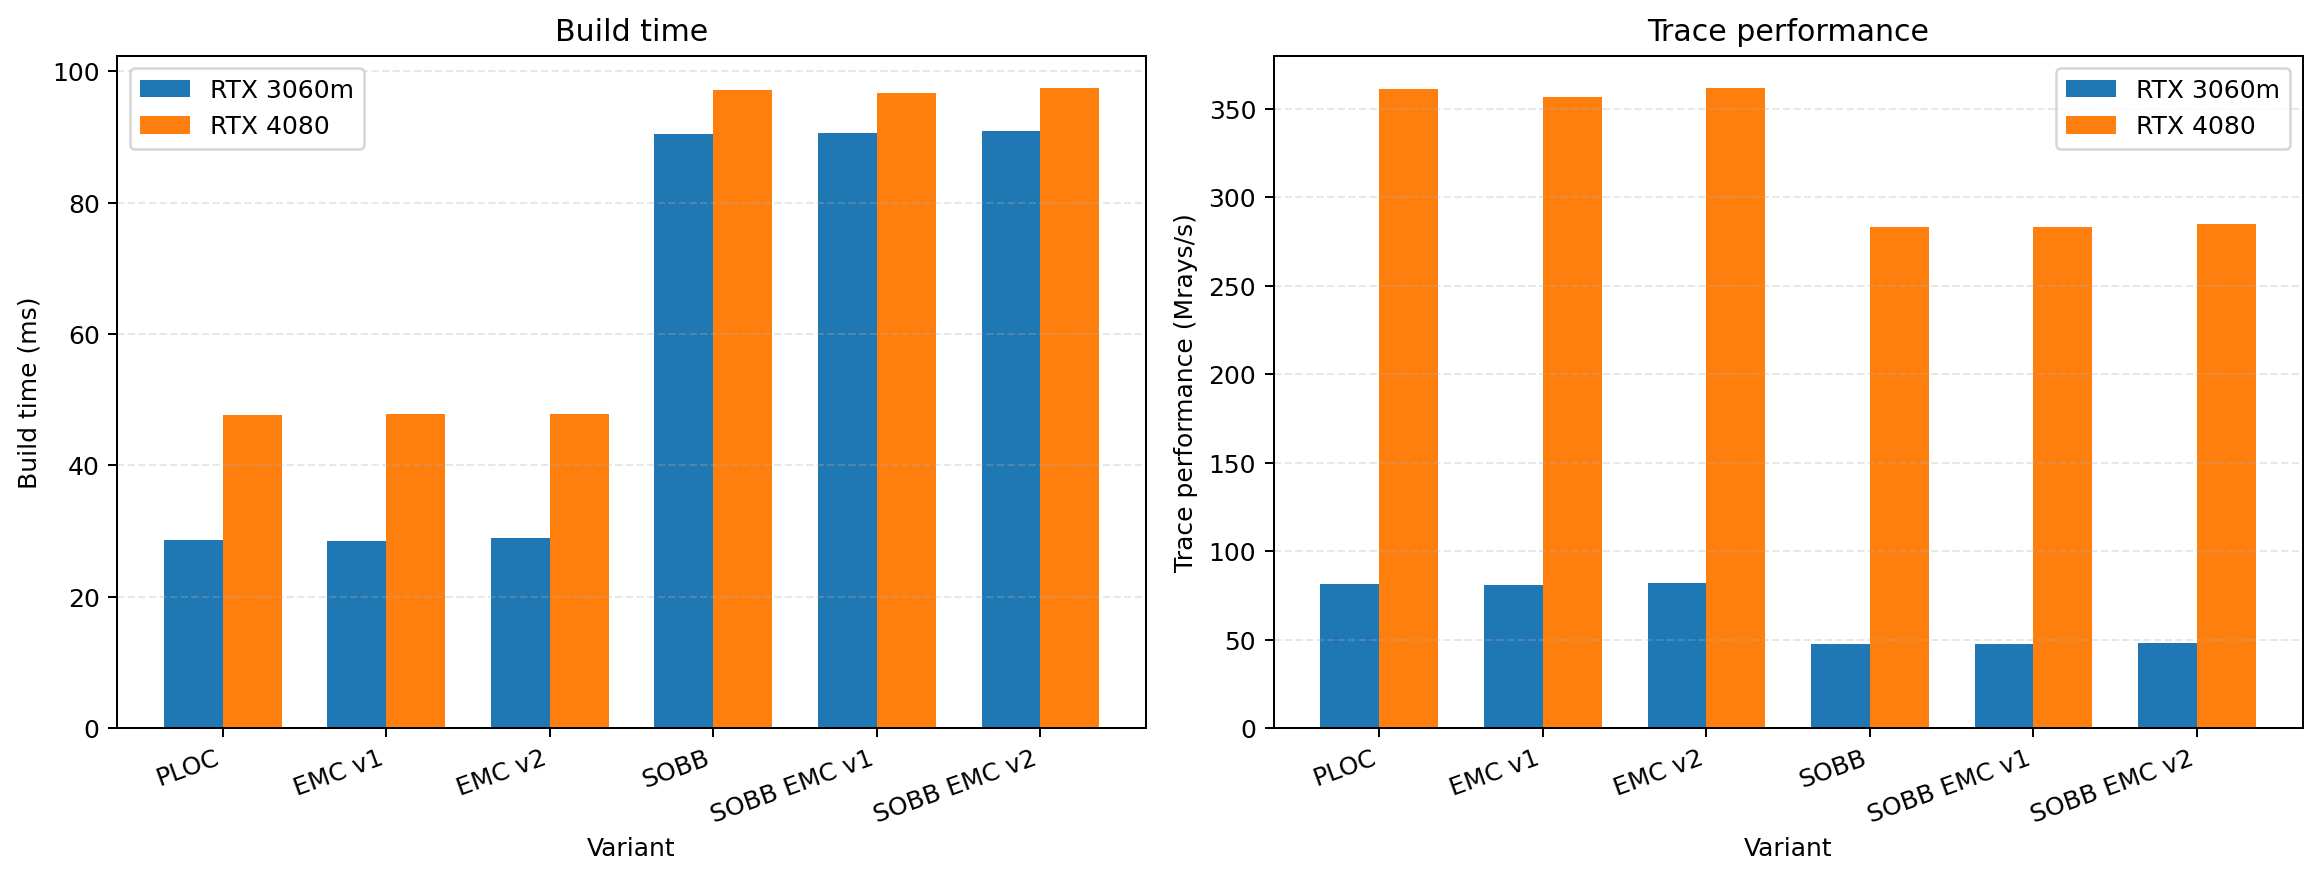
\includegraphics[width=0.95\textwidth]{images/results/graph_gpu_power_comparison.png}
\caption{Comparison of the raw power of the different GPUs and its effect on build time and trace performance.}
\label{fig:gpu-comparison-power}
\end{figure}

The experiments were conducted on two different systems to highlight the impact of hardware performance on the evaluated methods.

The first system was a laptop equipped with an Nvidia GeForce RTX 3060 Mobile GPU with 6~GB of VRAM and an AMD Ryzen 5 5600H CPU. The second system was a desktop workstation featuring an Nvidia GeForce RTX 4080 GPU with 16~GB of VRAM and an Intel Core i7-14700KF CPU.

This dual-platform evaluation allows for a comparison of both absolute performance and scalability across different hardware classes. The differences in BVH construction times and ray tracing throughput (measured in millions of rays per second, MRay/s) between the two systems are illustrated in Figure~\ref{fig:gpu-comparison-power}, where results are averaged across all scenes and camera configurations.

%---------------------------------------------------------------
\section{Scenes}

\begin{table}[!ht]
    \centering
    \small
    \resizebox{\textwidth}{!}{%
    \begin{tabular}{cccc}
        \hline
         Dragon & Hairball & PowerPlant & Rungholt \\
         800k & 2.9M & 12.8M & 5.8M \\
        
        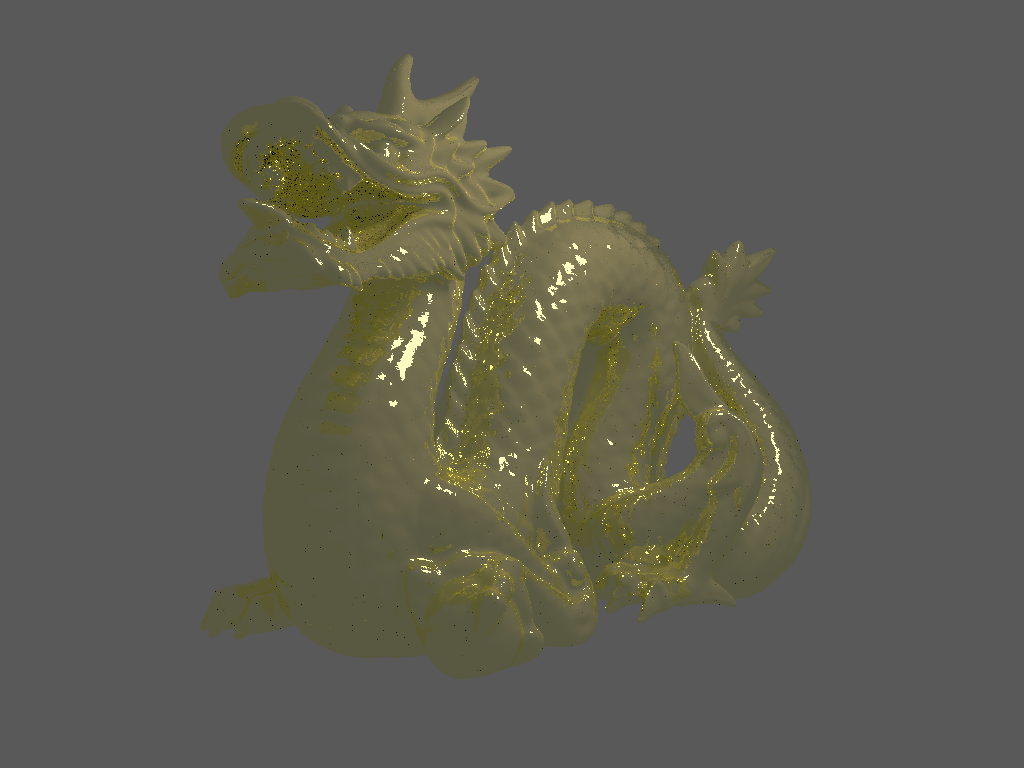
\includegraphics[width=0.25\textwidth]{images/renders/DragonCam0.png} &
        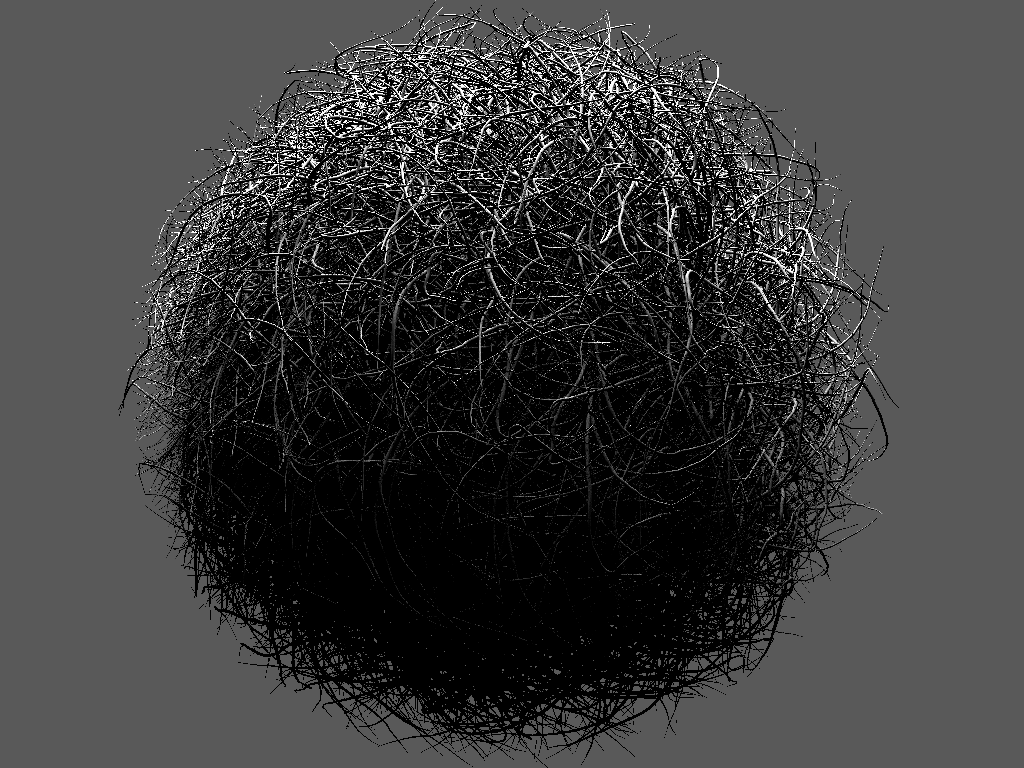
\includegraphics[width=0.25\textwidth]{images/renders/HairballCam0.png} &
        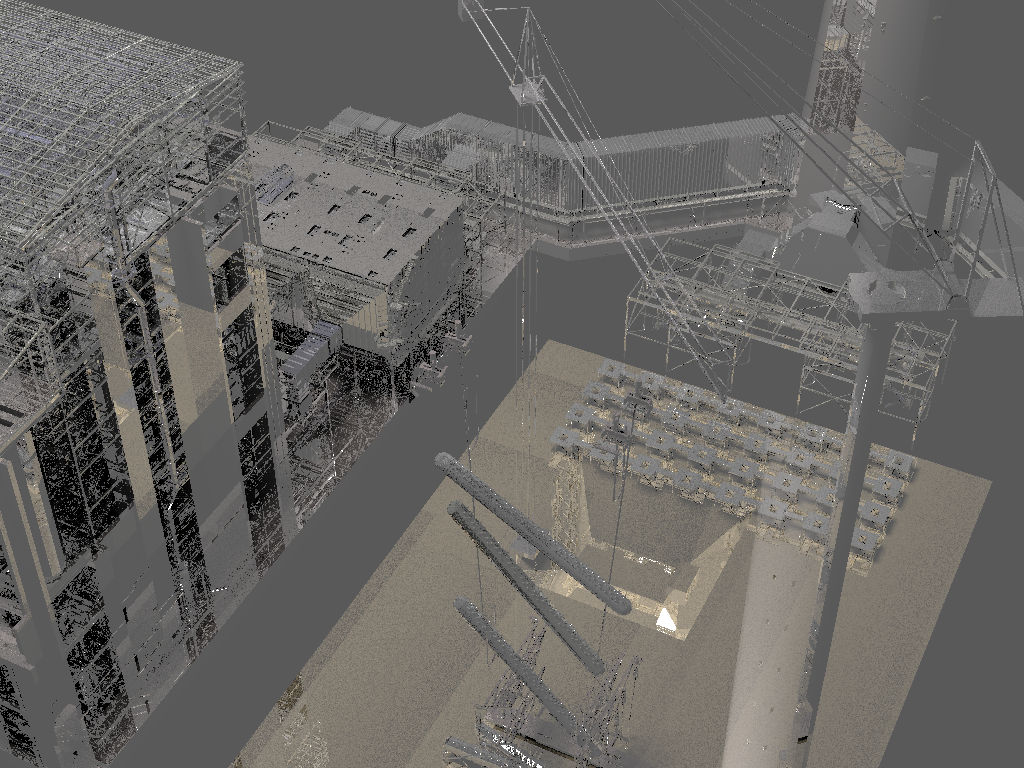
\includegraphics[width=0.25\textwidth]{images/renders/PowerPlantCam0.png} &
        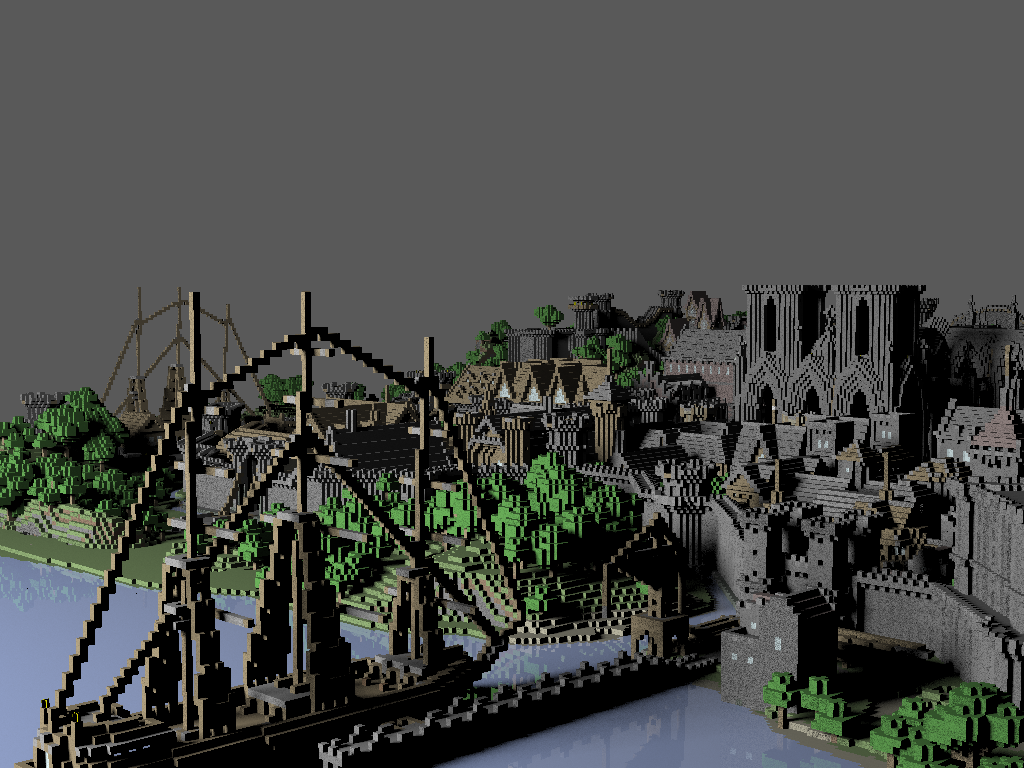
\includegraphics[width=0.25\textwidth]{images/renders/RungholtCam0.png} \\
        
        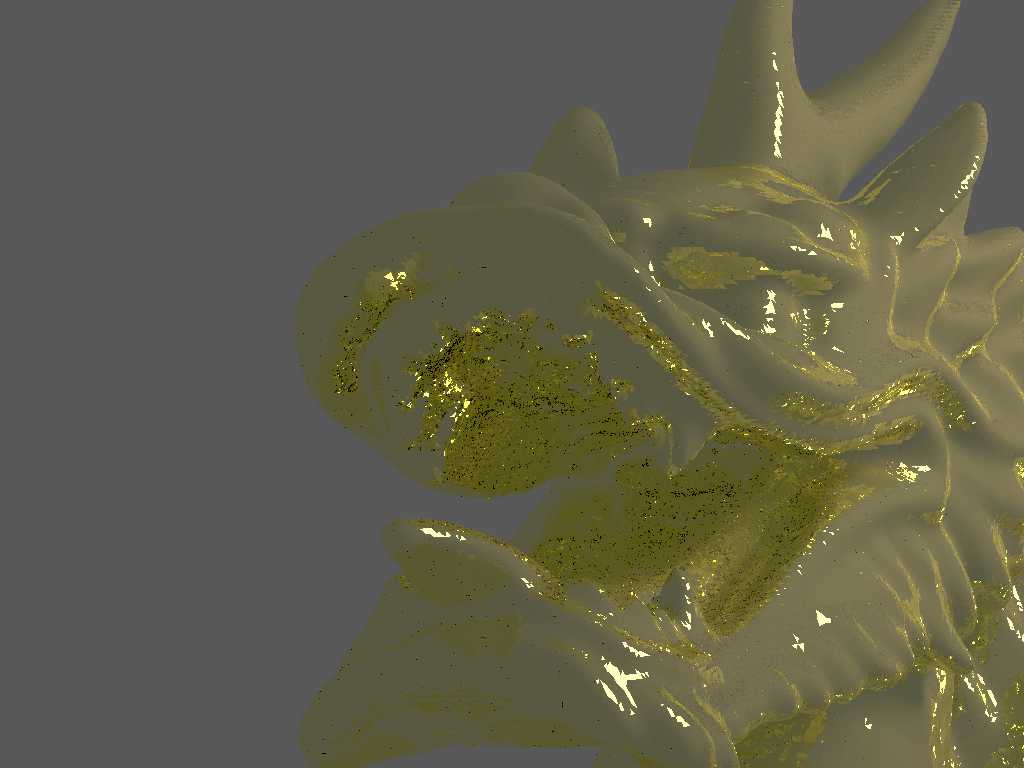
\includegraphics[width=0.25\textwidth]{images/renders/DragonCam1.png} &
        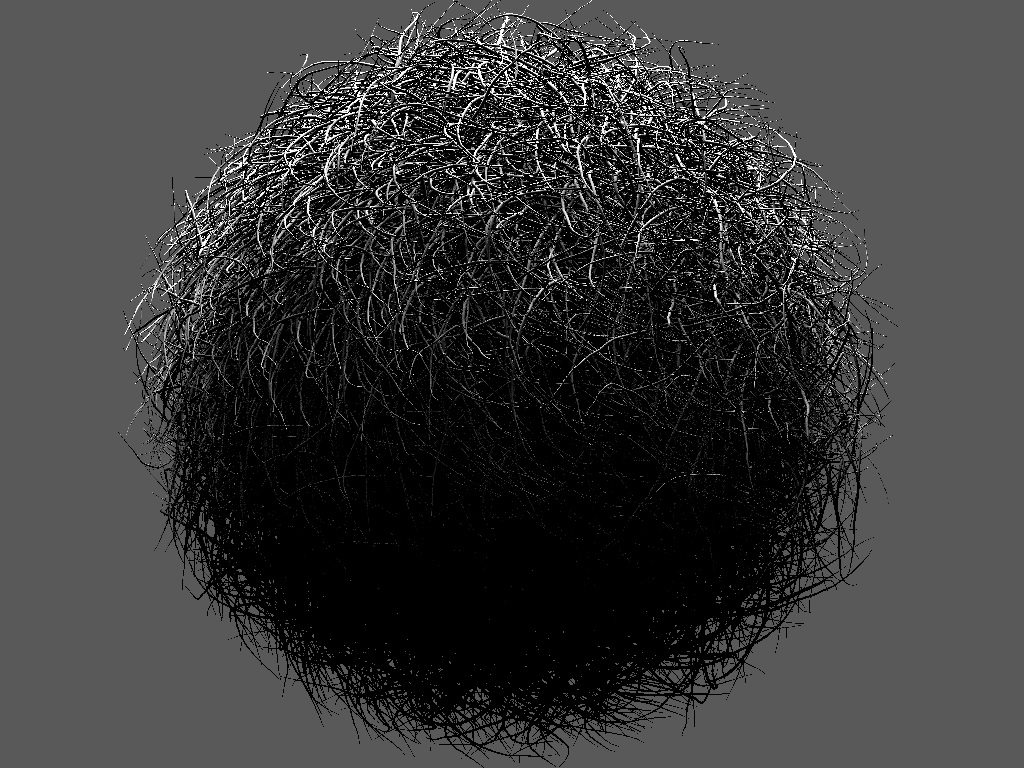
\includegraphics[width=0.25\textwidth]{images/renders/HairballCam1.png} &
        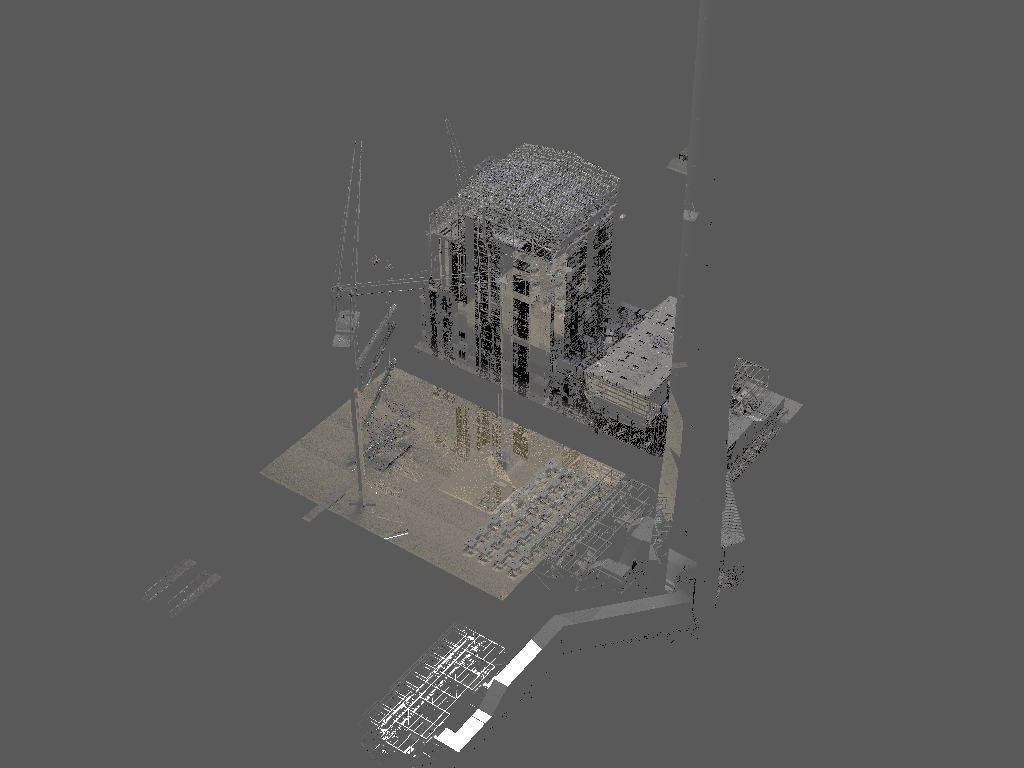
\includegraphics[width=0.25\textwidth]{images/renders/PowerPlantCam1.png} &
        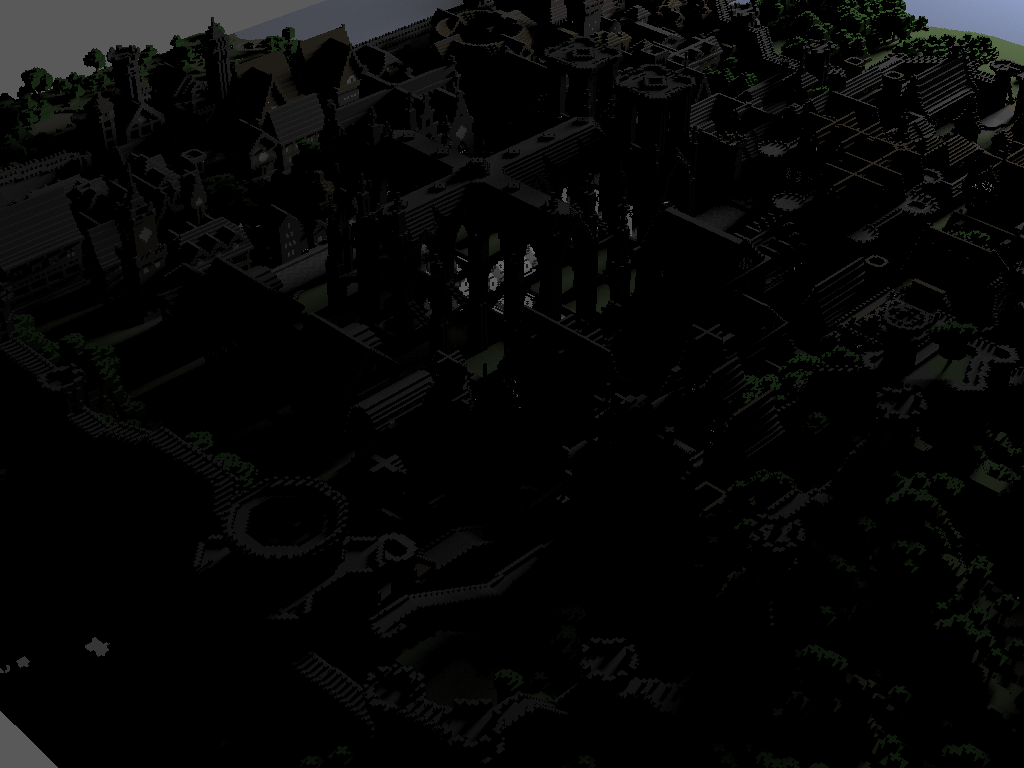
\includegraphics[width=0.25\textwidth]{images/renders/RungholtCam1.png} \\
        
        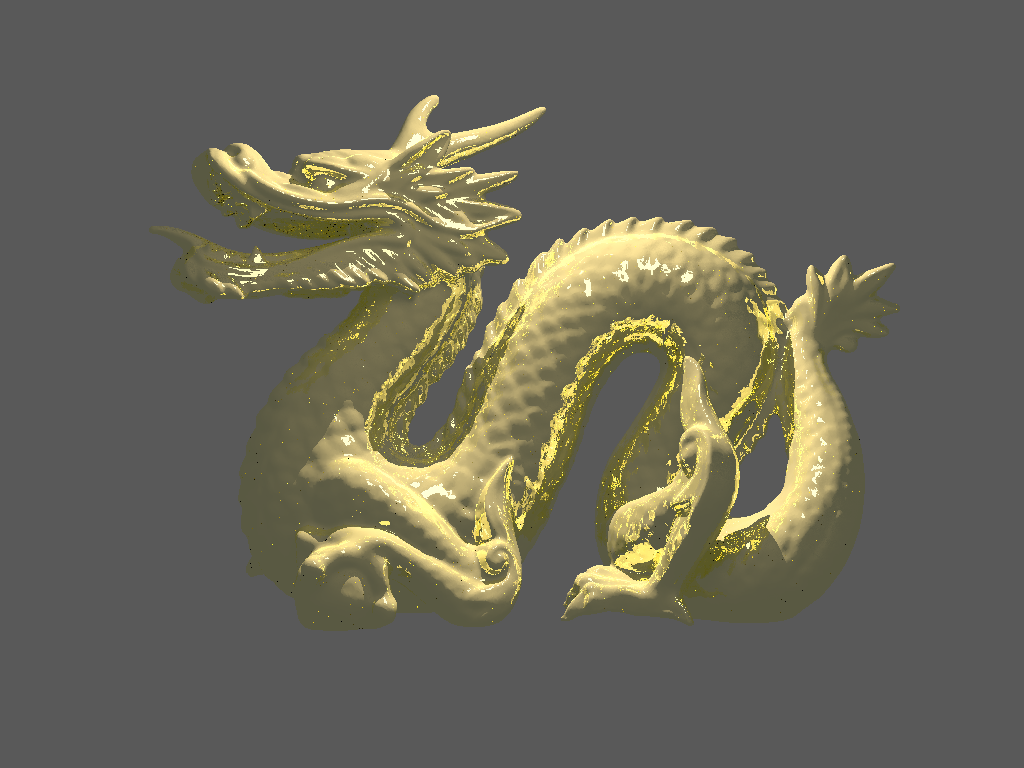
\includegraphics[width=0.25\textwidth]{images/renders/DragonCam2.png} &
        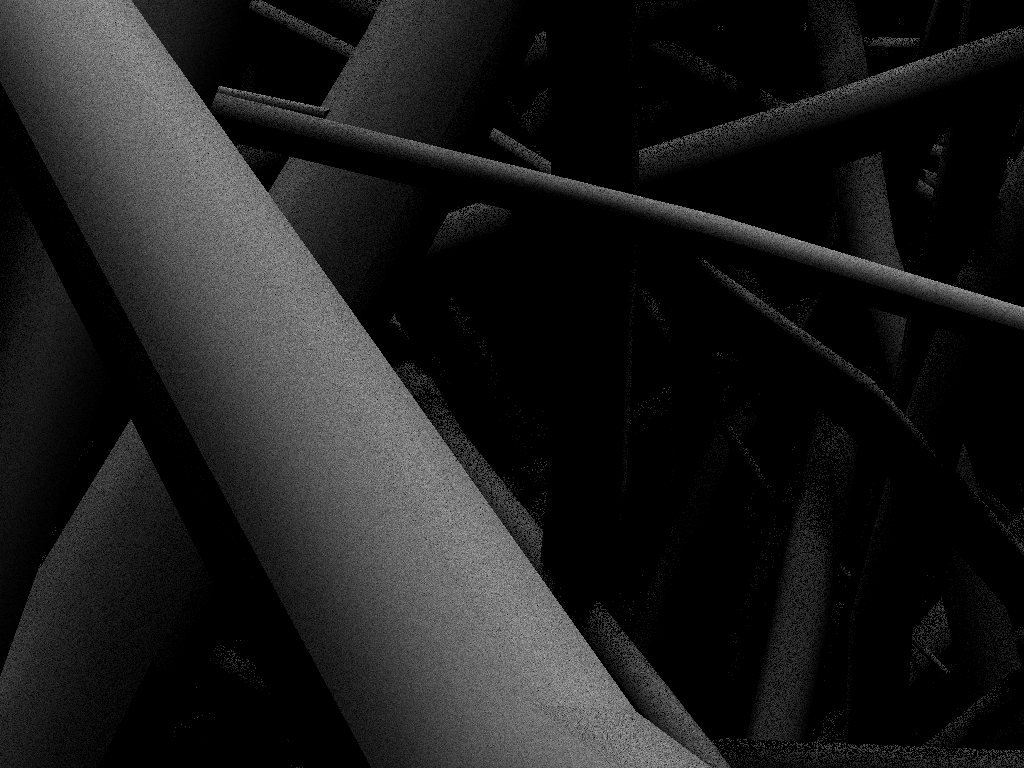
\includegraphics[width=0.25\textwidth]{images/renders/HairballCam2.png} &
        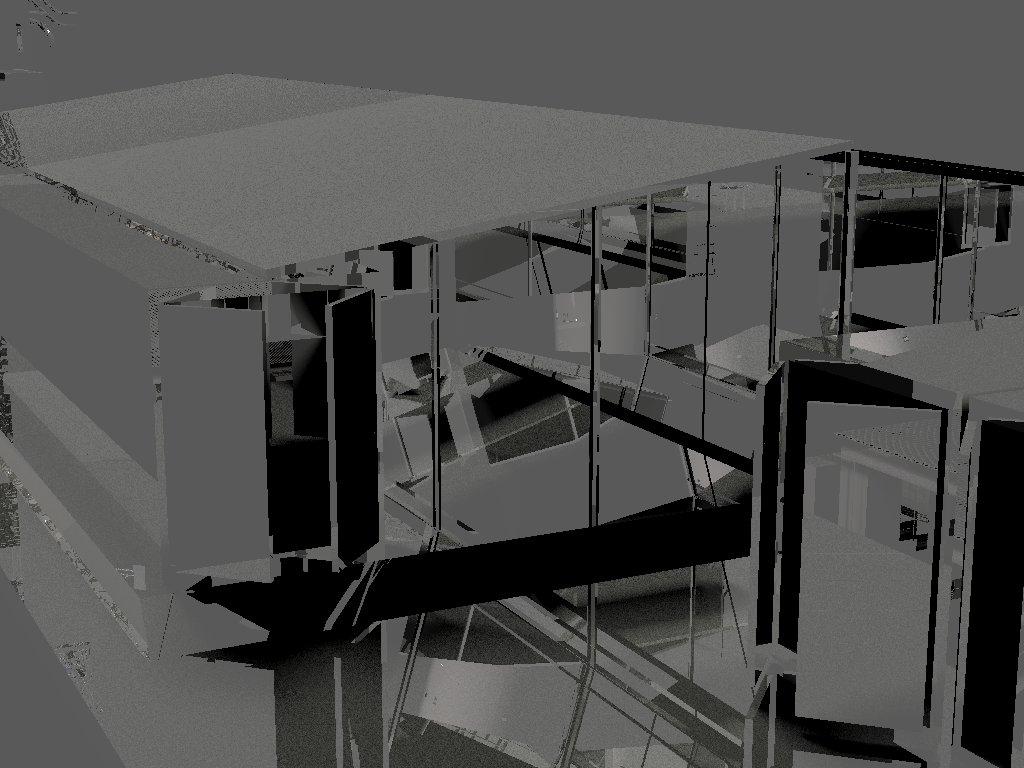
\includegraphics[width=0.25\textwidth]{images/renders/PowerPlantCam2.png} &
        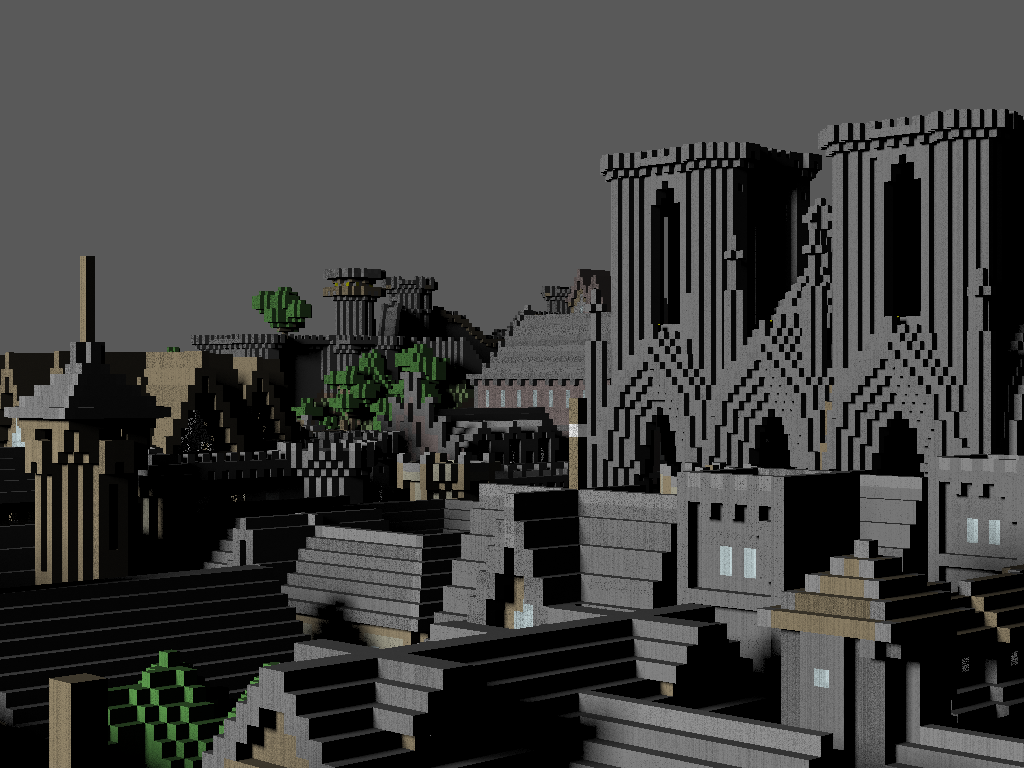
\includegraphics[width=0.25\textwidth]{images/renders/RungholtCam2.png} \\
         Skydemo & Sponza & Stegosaurus & Venlo \\
         3.7M & 262k & 5.7M & 1.3M \\
        
        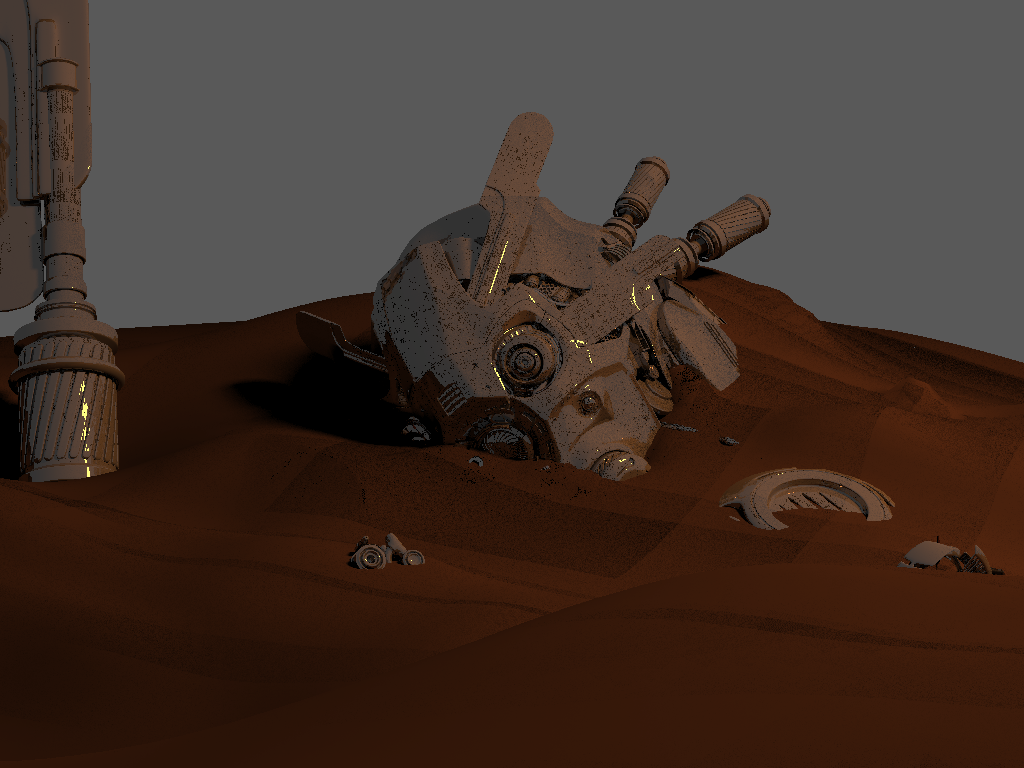
\includegraphics[width=0.25\textwidth]{images/renders/SkydemoCam0.png} &
        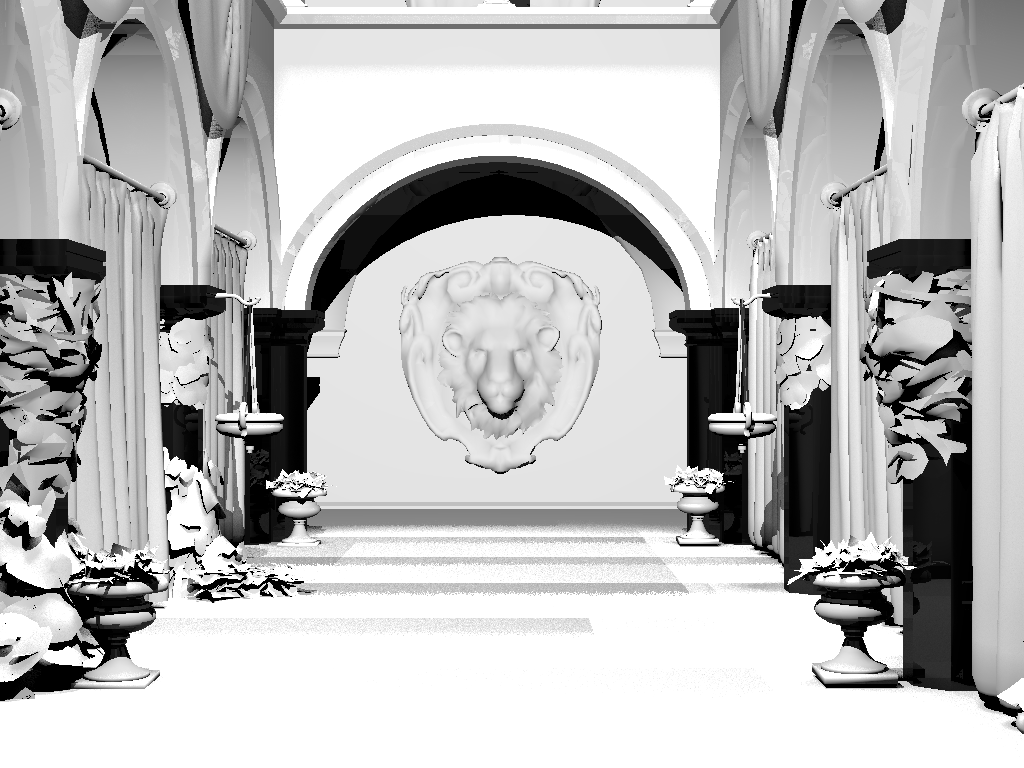
\includegraphics[width=0.25\textwidth]{images/renders/SponzaCam0.png} &
        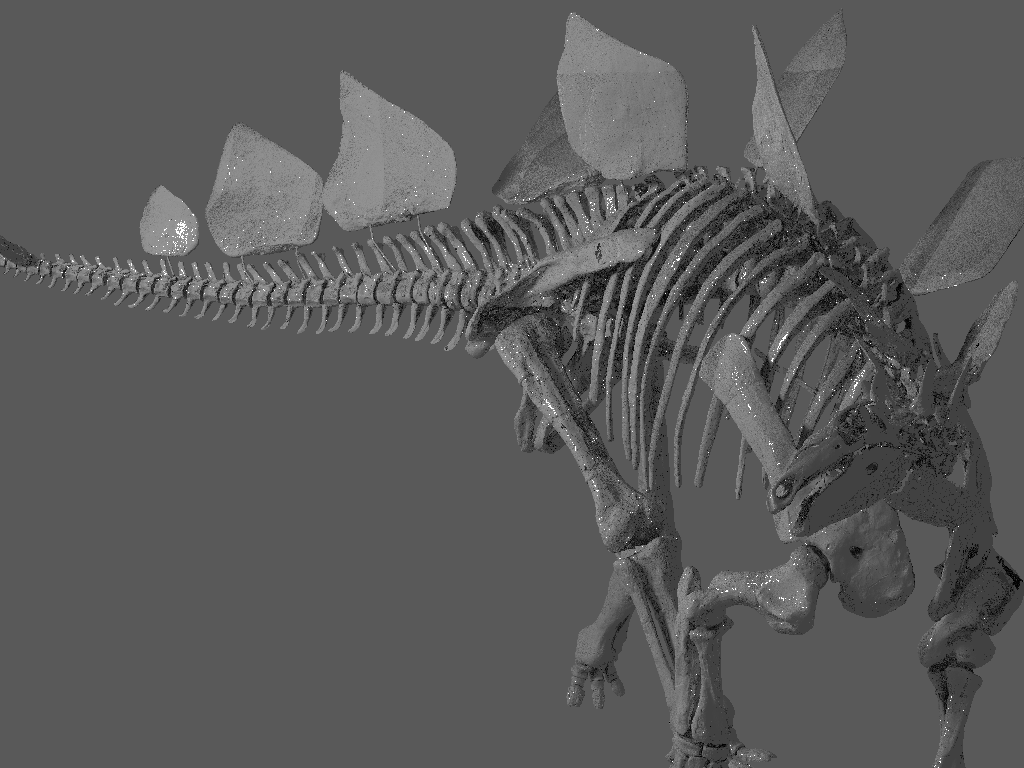
\includegraphics[width=0.25\textwidth]{images/renders/StegosaurusCam0.png} &
        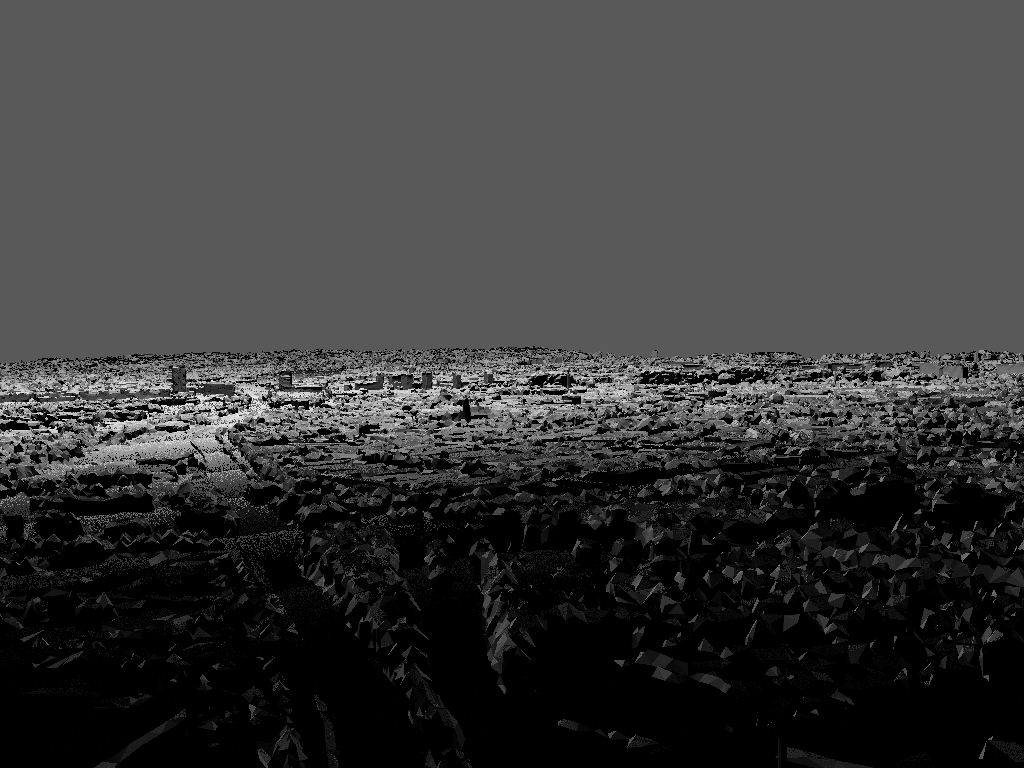
\includegraphics[width=0.25\textwidth]{images/renders/VenloCam0.png} \\
        
        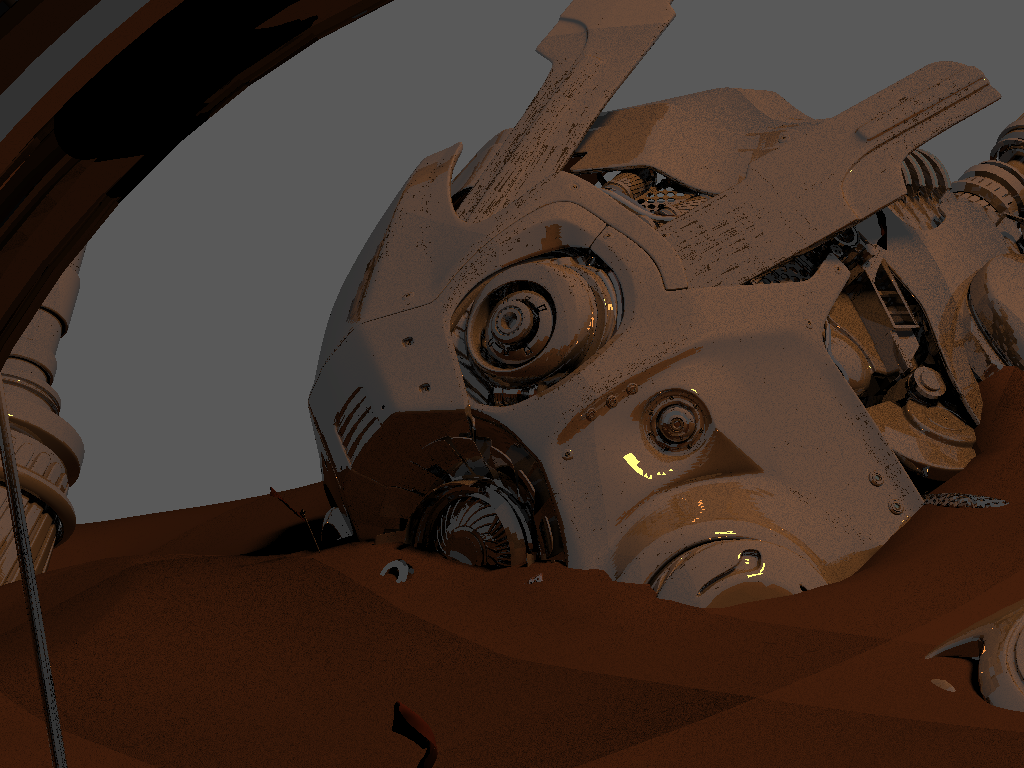
\includegraphics[width=0.25\textwidth]{images/renders/SkydemoCam1.png} &
        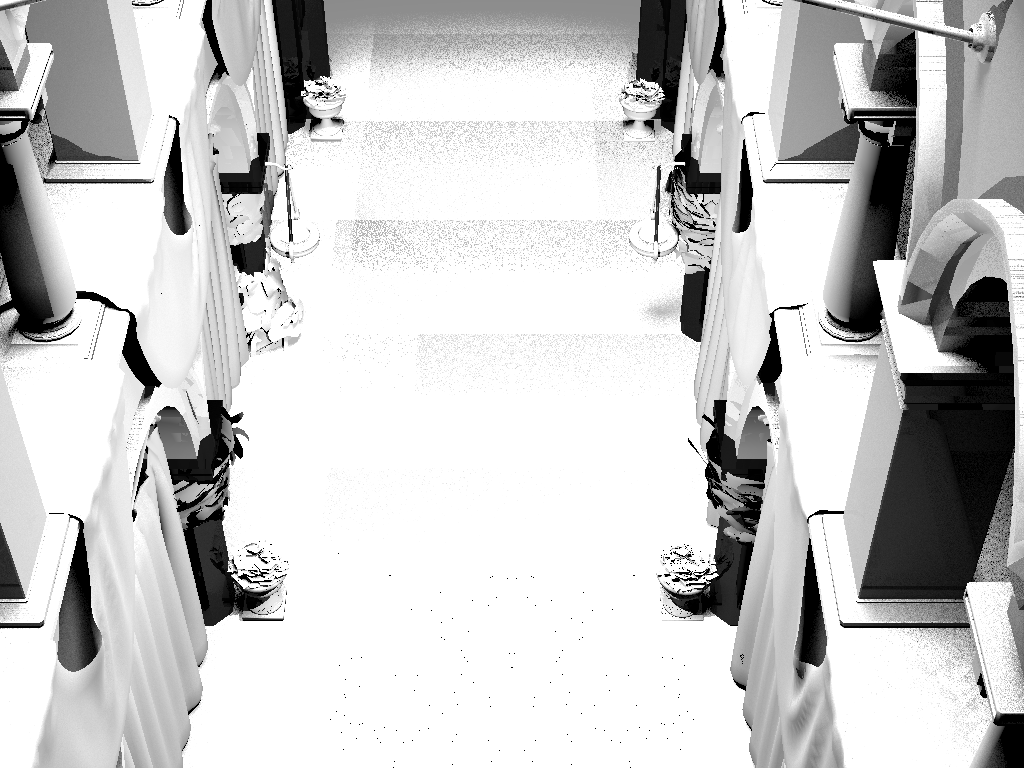
\includegraphics[width=0.25\textwidth]{images/renders/SponzaCam1.png} &
        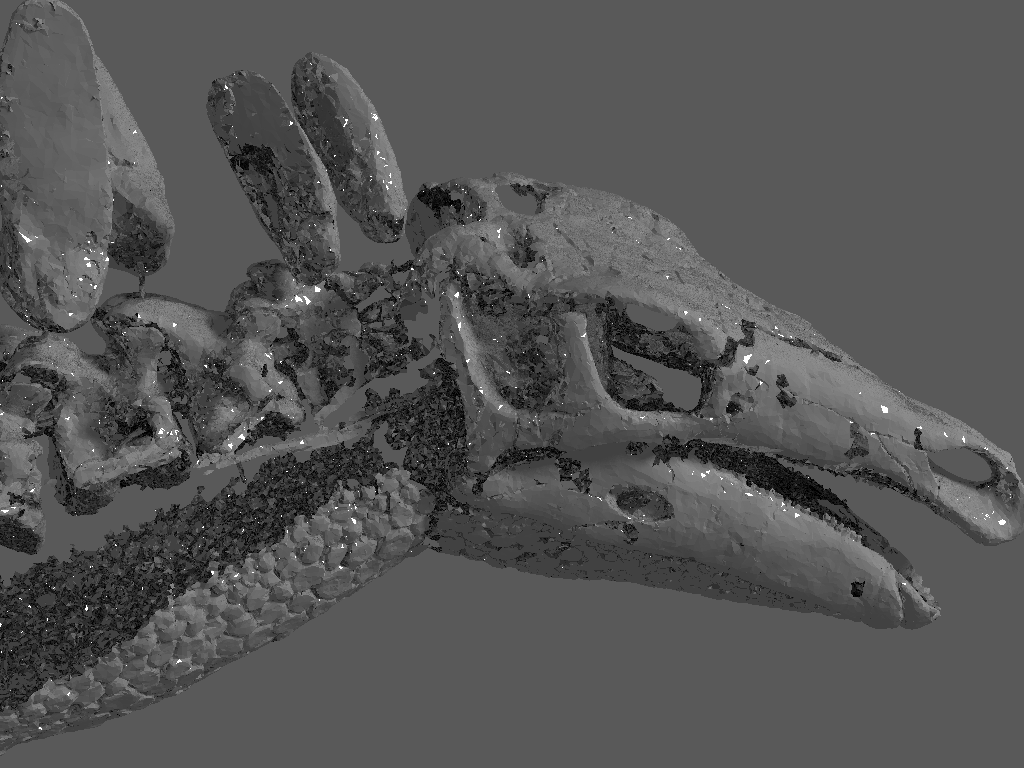
\includegraphics[width=0.25\textwidth]{images/renders/StegosaurusCam1.png} &
        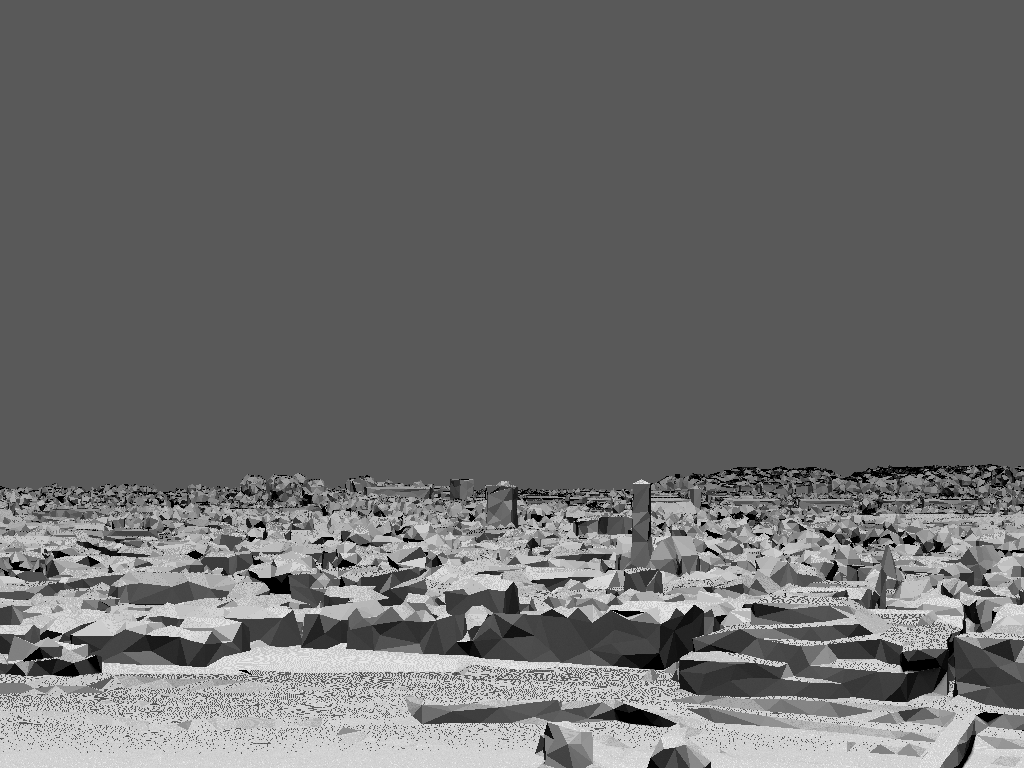
\includegraphics[width=0.25\textwidth]{images/renders/VenloCam1.png} \\
        
        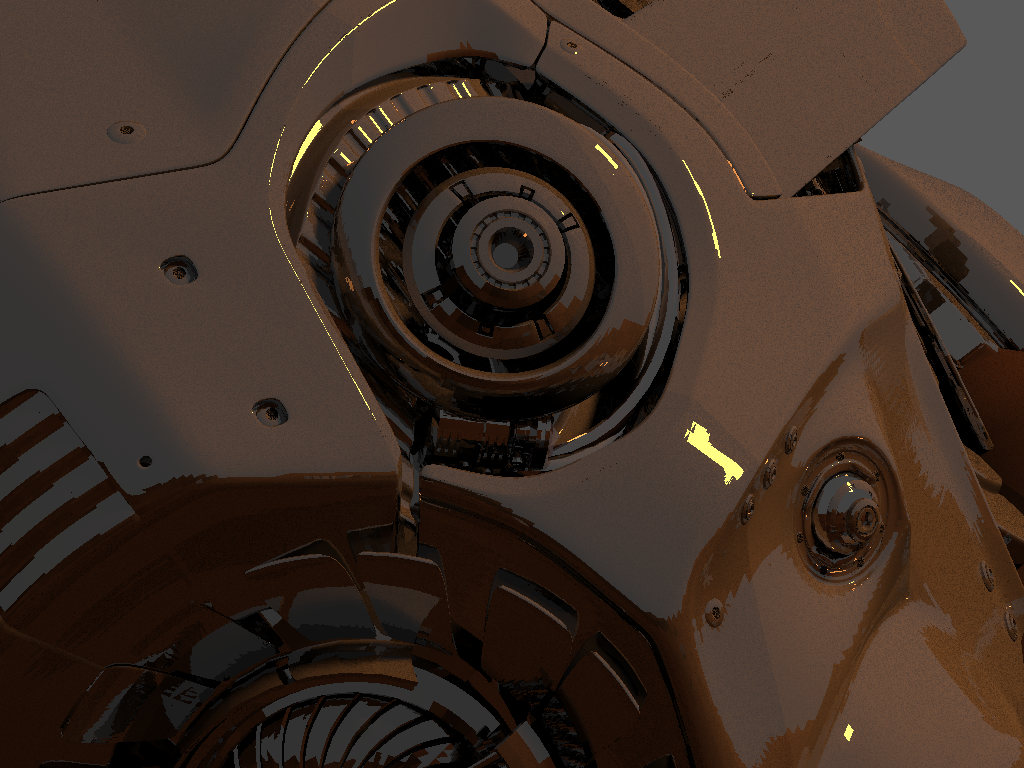
\includegraphics[width=0.25\textwidth]{images/renders/SkydemoCam2.png} &
        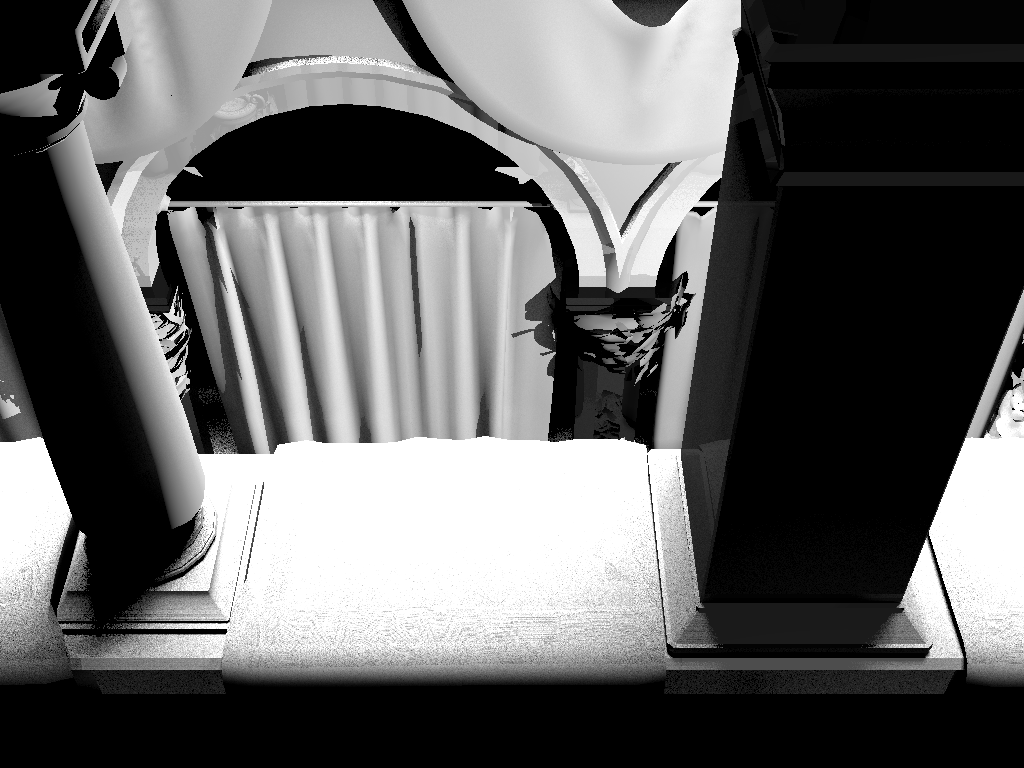
\includegraphics[width=0.25\textwidth]{images/renders/SponzaCam2.png} &
        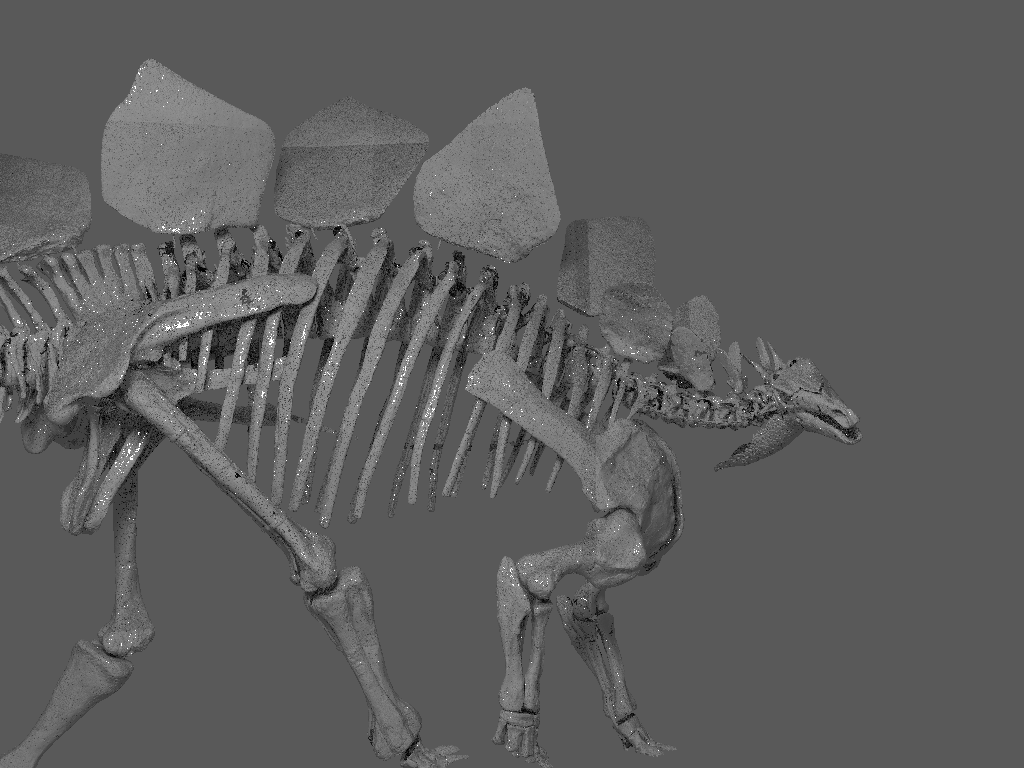
\includegraphics[width=0.25\textwidth]{images/renders/StegosaurusCam2.png} &
        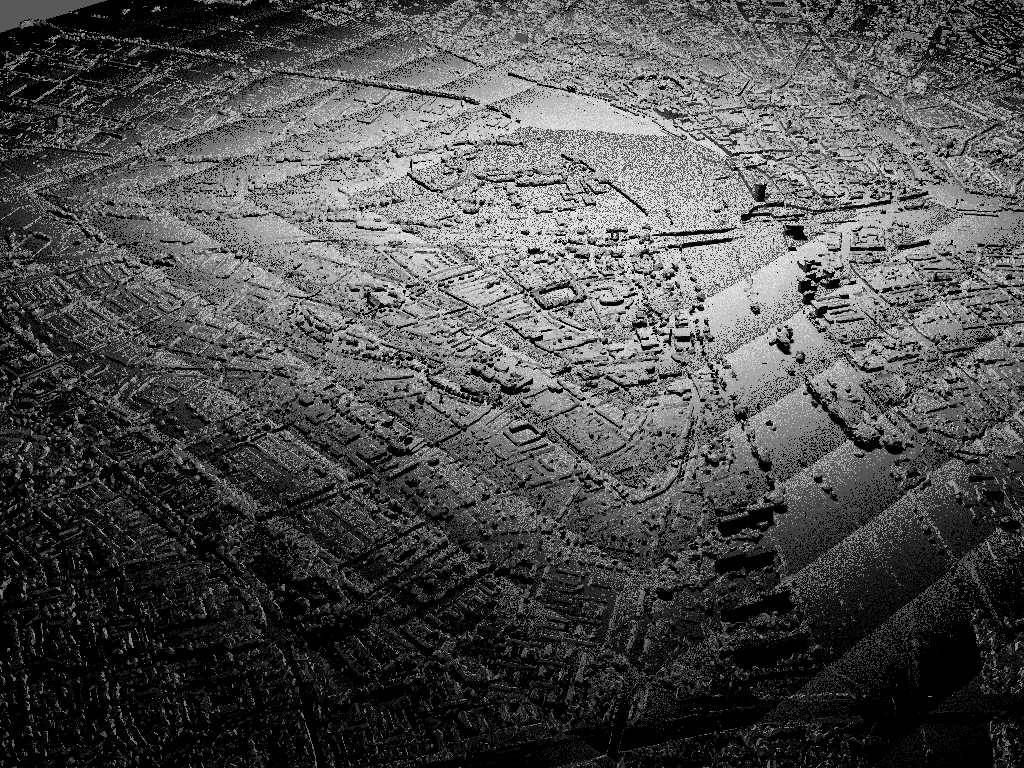
\includegraphics[width=0.25\textwidth]{images/renders/VenloCam2.png} \\
        \hline
    \end{tabular}
    }
    \caption{Rendered images of the 8 tested scenes in resolution $1024 \times 768$. Three representative views were used for each scene.}
    \label{tab:final-renders}
\end{table}

A total of 8 scenes were selected for evaluation, each rendered from 3 different camera viewpoints. These scenes were chosen to represent a diverse set of geometric complexity, spatial distribution, and visibility conditions, ensuring that the evaluated methods are tested under varying workloads.

For each scene and camera configuration, the rendering process generates a combination of primary rays, secondary rays (reflections and refractions), and shadow rays. The proportion of these ray types varies depending on scene composition, material properties, and camera placement, which directly influences the performance characteristics of the evaluated acceleration structures.

\begin{table}[!ht]
    \small
    \centering
    \resizebox{\textwidth}{!}{%
    \begin{tabular}{llccc}
        \hline
        Scene & Camera & Primary [Mrays] & Secondary [Mrays] & Shadow [Mrays] \\
        \hline

        \multirow{3}{*}{\shortstack{Dragon \\ \# of triangles: 800k}}
        & cam0 & 25.17 (30.95\%) & 11.23 (13.81\%) & 44.92 (55.24\%) \\
        & cam1 & 25.17 (16.87\%) & 24.81 (16.63\%) & 99.23 (66.51\%) \\
        & cam2 & 25.17 (27.97\%) & 10.80 (12.00\%) & 54.01 (60.02\%) \\

        \hline
        \multirow{3}{*}{\shortstack{Hairball \\ \# of triangles: 2.9M}}
        & cam0 & 25.17 (34.06\%) & 0.00 (0.00\%) & 48.72 (65.94\%) \\
        & cam1 & 25.17 (33.65\%) & 0.00 (0.00\%) & 49.63 (66.35\%) \\
        & cam2 & 25.17 (20.00\%) & 0.00 (0.00\%) & 100.66 (80.00\%) \\

        \hline
        \multirow{3}{*}{\shortstack{PowerPlant \\ \# of triangles: 12.8M}}
        & cam0 & 25.17 (8.69\%) & 52.86 (18.26\%) & 211.45 (73.05\%) \\
        & cam1 & 25.17 (27.00\%) & 13.61 (14.60\%) & 54.44 (58.40\%) \\
        & cam2 & 25.17 (5.34\%) & 89.30 (18.93\%) & 357.20 (75.73\%) \\

        \hline
        \multirow{3}{*}{\shortstack{Rungholt \\ \# of triangles: 5.8M}}
        & cam0 & 25.17 (28.71\%) & 1.73 (1.97\%) & 60.77 (69.32\%) \\
        & cam1 & 25.17 (19.74\%) & 1.02 (0.80\%) & 101.29 (79.46\%) \\
        & cam2 & 25.17 (26.12\%) & 0.46 (0.48\%) & 70.73 (73.40\%) \\

        \hline
        \multirow{3}{*}{\shortstack{Skydemo \\ \# of triangles: 3.7M}}
        & cam0 & 25.17 (21.71\%) & 7.56 (6.52\%) & 83.20 (71.77\%) \\
        & cam1 & 25.17 (14.22\%) & 21.90 (12.37\%) & 129.90 (73.41\%) \\
        & cam2 & 25.17 (9.84\%) & 40.41 (15.80\%) & 190.15 (74.36\%) \\

        \hline
        \multirow{3}{*}{\shortstack{Sponza \\ \# of triangles: 262k}}
        & cam0 & 25.17 (10.92\%) & 13.27 (5.76\%) & 191.93 (83.32\%) \\
        & cam1 & 25.17 (12.27\%) & 9.14 (4.45\%) & 170.77 (83.27\%) \\
        & cam2 & 25.17 (11.63\%) & 10.92 (5.05\%) & 180.35 (83.33\%) \\

        \hline
        \multirow{3}{*}{\shortstack{Stegosaurus \\ \# of triangles: 5.7M}}
        & cam0 & 25.17 (24.78\%) & 15.28 (15.04\%) & 61.11 (60.18\%) \\
        & cam1 & 25.17 (15.32\%) & 27.82 (16.94\%) & 111.28 (67.74\%) \\
        & cam2 & 25.17 (23.77\%) & 16.14 (15.25\%) & 64.56 (60.98\%) \\

        \hline
        \multirow{3}{*}{\shortstack{Venlo \\ \# of triangles: 1.3M}}
        & cam0 & 25.17 (31.64\%) & 0.00 (0.00\%) & 54.36 (68.36\%) \\
        & cam1 & 25.17 (39.93\%) & 0.00 (0.00\%) & 37.86 (60.07\%) \\
        & cam2 & 25.17 (20.04\%) & 0.00 (0.00\%) & 100.44 (79.96\%) \\

        \hline
    \end{tabular}
    }
    \caption{Ray distribution per scene and camera. Ray counts are shown in millions (Mrays), with percentage share in parentheses.}
    \label{tab:ray-distribution}
\end{table}

To provide visual context, the final rendered images of all scenes are presented in Table~\ref{tab:final-renders}. Additionally, a detailed breakdown of ray counts, including their absolute values and relative percentages of the total ray count, is provided in Table~\ref{tab:ray-distribution} along with the triangle counts for each scene. This information is important for understanding how different ray types contribute to the overall workload and how they may impact traversal performance.

As in the overall experimental setup, each scene and camera combination was evaluated 5 times, and the median value was used to mitigate the effect of random performance fluctuations.

Most of the scenes are courtesy of Morgan McGuire's archive \cite{McGuire2017}. The Stegosaurus scene was taken from the Smithsonian institution's 3D render archive \cite{si}. The Skydemo scene is part of the Blender demo files \cite{blender_demo}.

%---------------------------------------------------------------
\clearpage
\newpage
\section{Results}

\begin{figure}[h!tb]
\centering
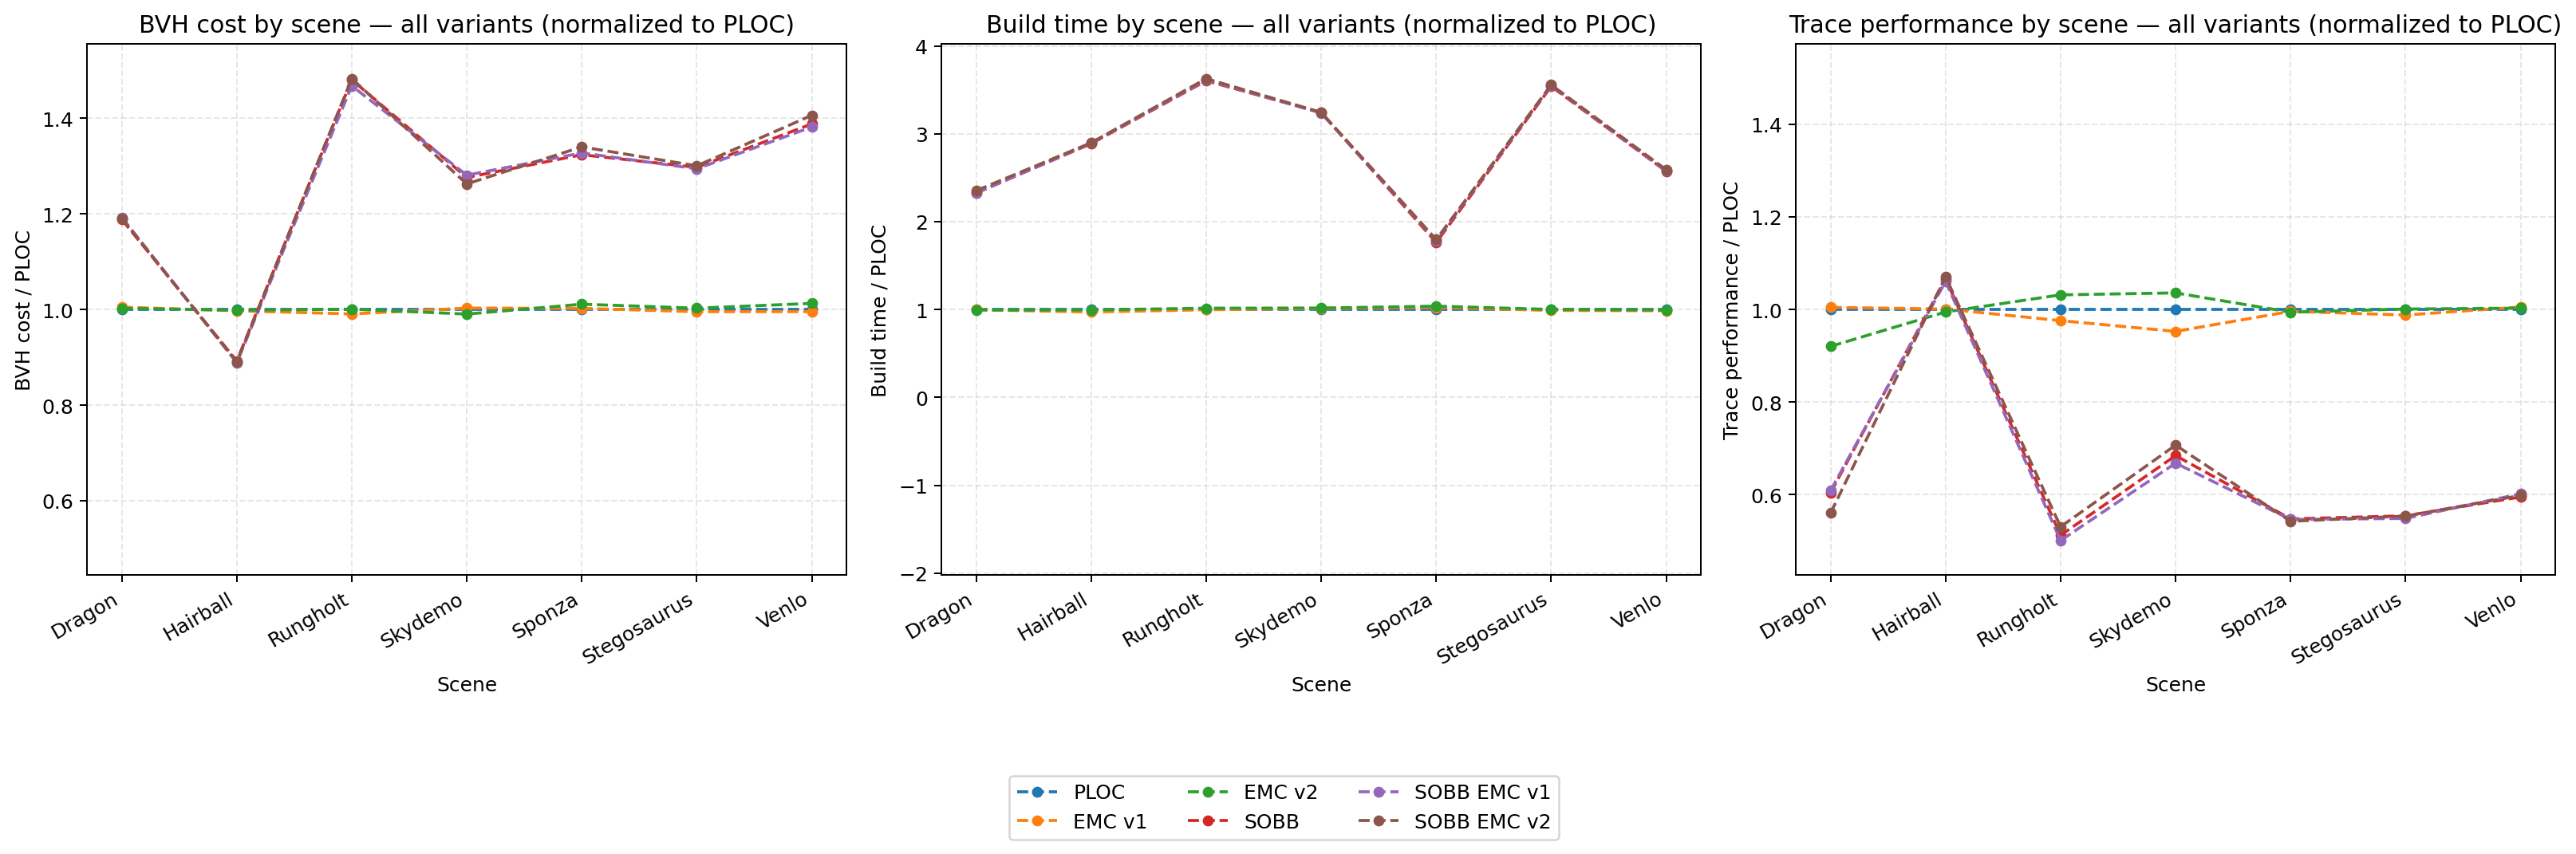
\includegraphics[width=0.95\textwidth]{images/results/rtx3060mobile/graph_scene_statistics_all_variants_normalized.png}
\caption{BVH cost, build time (in ms) and traversal performance (in Mrays/s) per scene, relative to the PLOC variant. Nvidia RTX 3060 Mobile.}
\label{fig:scene-statistics-all-variants-3060}
\end{figure}

\begin{figure}[h!tb]
\centering

\includegraphics[width=0.95\textwidth]{images/results/rtx4080/graph_scene_statistics_all_variants_normalized.png}
\caption{BVH cost, build time (in ms) and traversal performance (in Mrays/s) per scene, relative to the PLOC variant. Nvidia RTX 4080.}
\label{fig:scene-statistics-all-variants-4080}
\end{figure}

Figures~\ref{fig:scene-statistics-all-variants-3060} and \ref{fig:scene-statistics-all-variants-4080} present an overview of the measured results for the Nvidia GeForce RTX 3060 Mobile and Nvidia GeForce RTX 4080, respectively. These figures summarize three key metrics: BVH cost, construction time (in milliseconds), and traversal performance (in millions of rays per second, MRay/s). For clarity, all values are expressed relative to the baseline PLOC variant.

Each data point represents an average across all scenes and camera configurations. While this aggregated view provides a general comparison of the evaluated methods, it also reveals that some variants exhibit very similar performance characteristics. In particular, the PLOC, EMC v1, and EMC v2 variants tend to produce closely clustered results, as do the SOBB-based variants. As a consequence, differences between individual methods are less distinguishable in these combined plots.

\begin{figure}[h!tb]
\centering
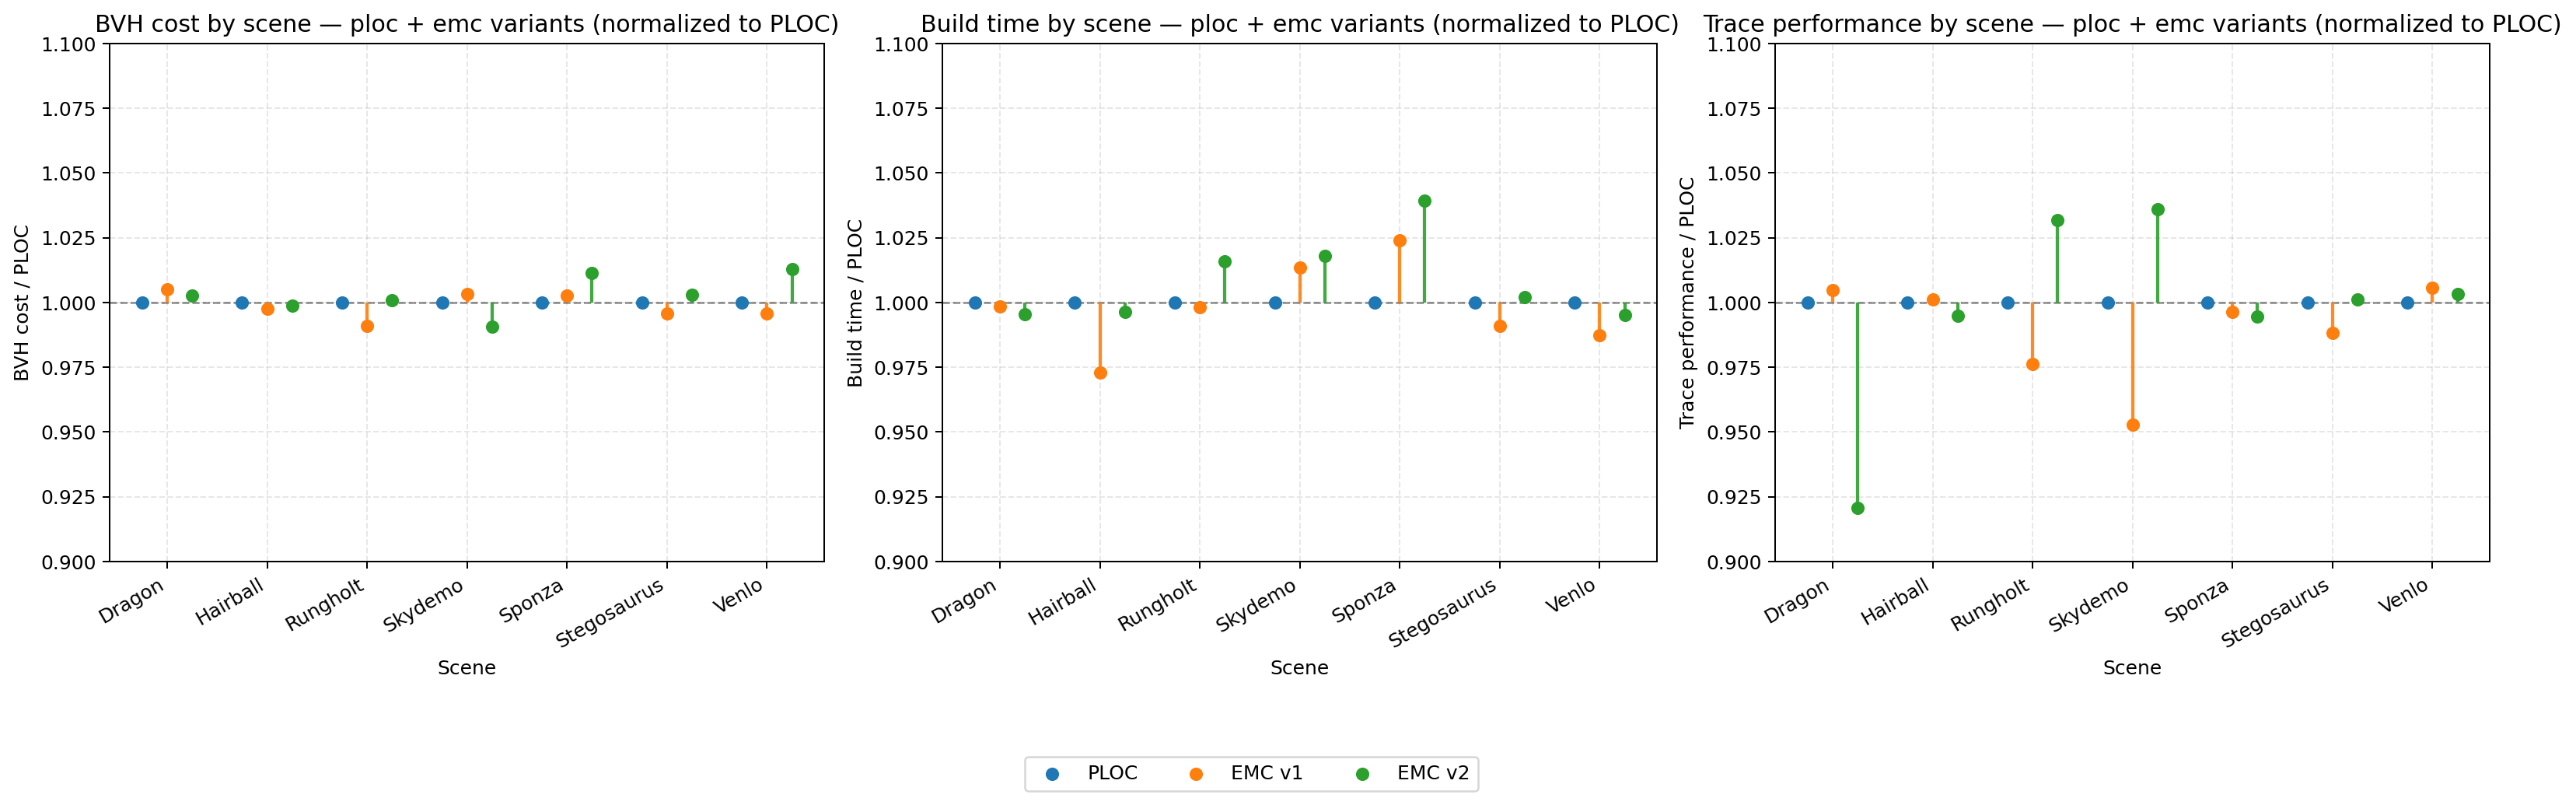
\includegraphics[width=0.95\textwidth]{images/results/rtx3060mobile/graph_scene_statistics_ploc_emc_normalized.png}
\caption{BVH cost, build time (in ms) and traversal performance (in Mrays/s) per scene for PLOC, PLOC EMC v1 and PLOC EMC v2 variants, relative to the PLOC variant. Nvidia RTX 3060 Mobile.}
\label{fig:scene-statistics-emc-3060}
\end{figure}

\begin{figure}[h!tb]
\centering

\includegraphics[width=0.95\textwidth]{images/results/rtx4080/graph_scene_statistics_ploc_emc_normalized.png}
\caption{BVH cost, build time (in ms) and traversal performance (in Mrays/s) per scene for PLOC, PLOC EMC v1 and PLOC EMC v2 variants, relative to the PLOC variant. Nvidia RTX 4080.}
\label{fig:scene-statistics-emc-4080}
\end{figure}

To improve readability and enable a more detailed comparison, the results are further divided into two groups. Figures~\ref{fig:scene-statistics-emc-3060} and \ref{fig:scene-statistics-emc-4080} focus on the baseline and EMC-enhanced variants (PLOC, EMC v1, EMC v2), with all values normalized relative to the PLOC baseline. Similarly, Figures~\ref{fig:scene-statistics-sobb-3060} and \ref{fig:scene-statistics-sobb-4080} present the SOBB-based variants (SOBB, SOBB EMC v1, SOBB EMC v2), normalized relative to the SOBB baseline.

\begin{figure}[h!tb]
\centering
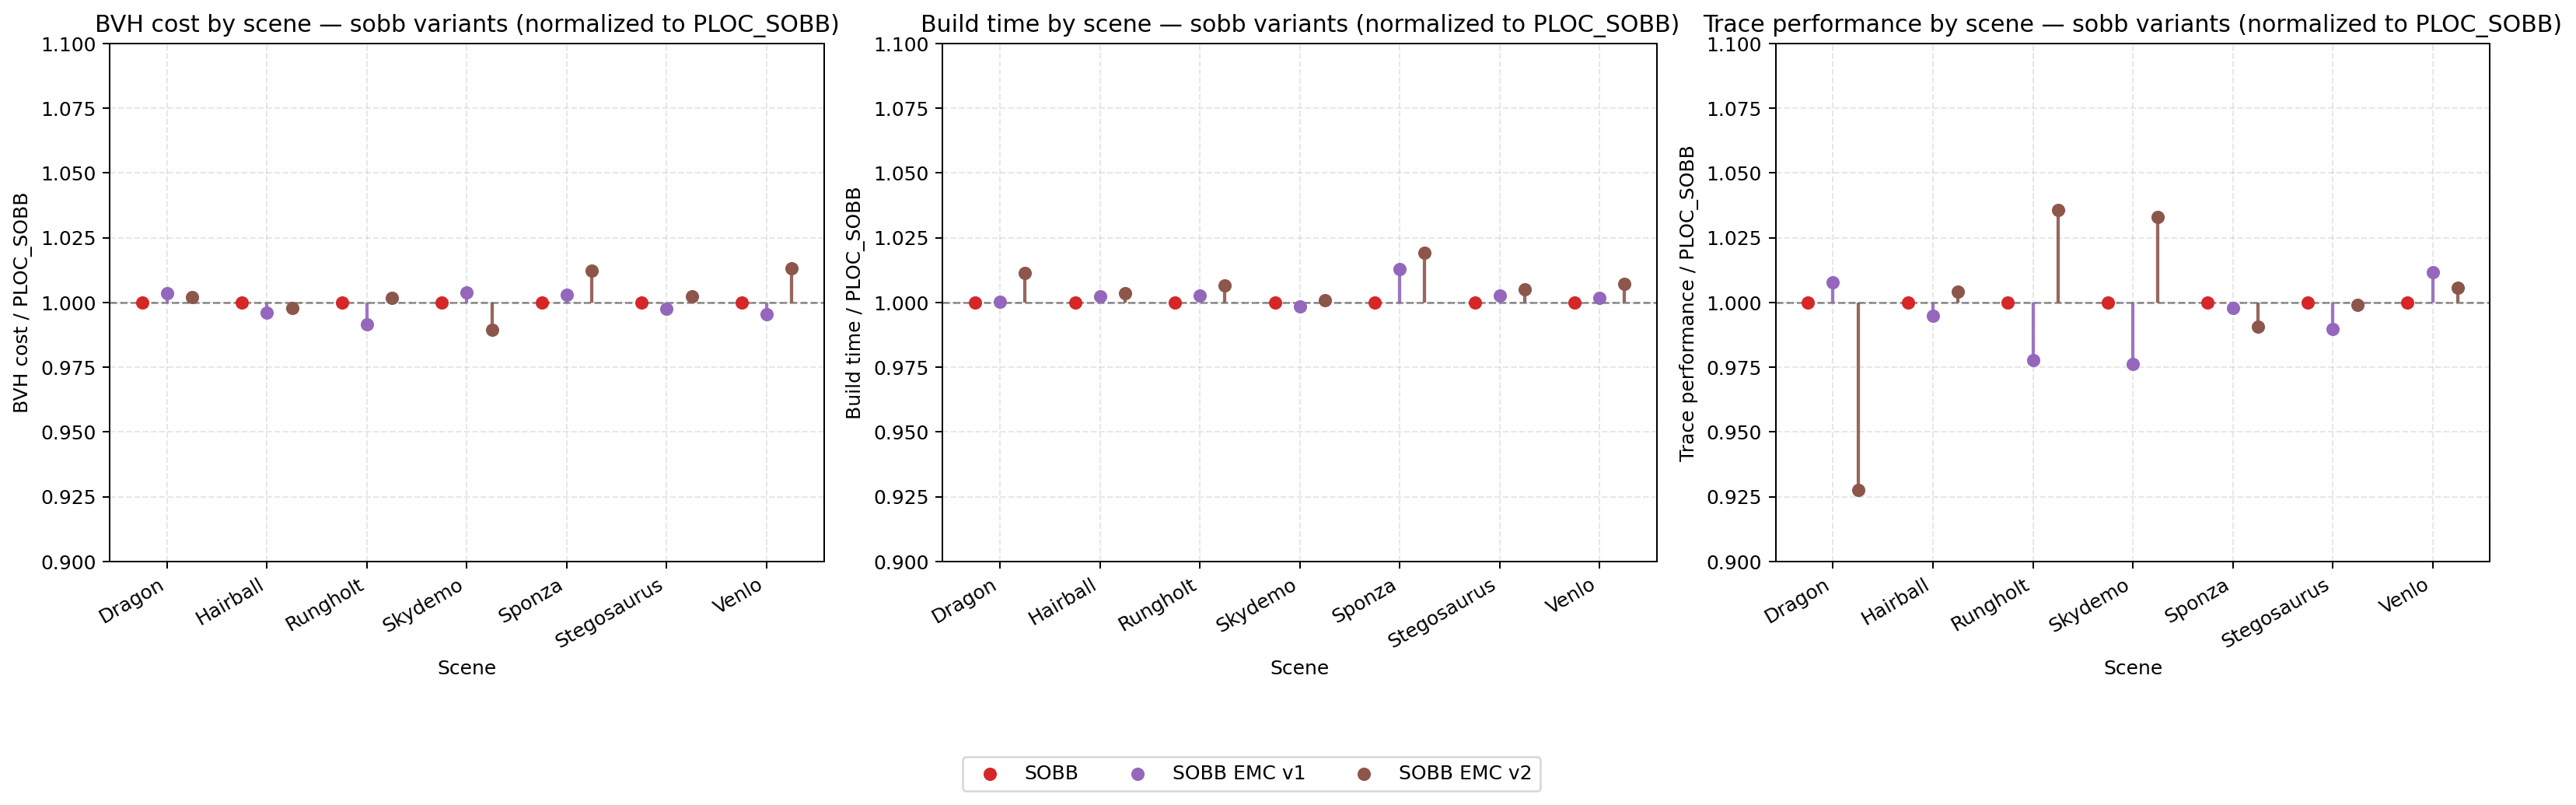
\includegraphics[width=0.95\textwidth]{images/results/rtx3060mobile/graph_scene_statistics_sobb_normalized.png}
\caption{BVH cost, build time (in ms) and traversal performance (in Mrays/s) per scene for SOBB, SOBB EMC v1 and SOBB EMC v2 variants, relative to the SOBB variant. Nvidia RTX 3060 Mobile.}
\label{fig:scene-statistics-sobb-3060}
\end{figure}

\begin{figure}[h!tb]
\centering

\includegraphics[width=0.95\textwidth]{images/results/rtx4080/graph_scene_statistics_sobb_normalized.png}
\caption{BVH cost, build time (in ms) and traversal performance (in Mrays/s) per scene for SOBB, SOBB EMC v1 and SOBB EMC v2 variants, relative to the SOBB variant. Build time for the Sponza scene for the SOBB EMC v2 variant is an outlier and thus the graph is not scaled to see its true values. Nvidia RTX 4080.}
\label{fig:scene-statistics-sobb-4080}
\end{figure}

This separation allows for a clearer comparison of incremental improvements introduced by the individual techniques. In particular, it highlights the relative impact of Extended Morton Codes within the same bounding volume representation, as well as their interaction with alternative bounding volumes.

The following subsections analyze each of the measured metrics in detail. In addition to the graphical summaries, precise numerical results are provided in tabular form to support a more rigorous comparison.

%---------------------------------------------------------------
\subsection{Build time}
\label{sec:build-time}

\begin{figure}[h!tb]
\centering

\includegraphics[width=0.95\textwidth]{images/results/rtx4080/graph_build_time_breakdown_stacked.png}
\caption{Breakdown of the total build time (in ms) for different variants. Only explicitly measured parts are shown, omitting minor overheads. The times for different stages are similar on both GPUs (percentage-wise).}
\label{fig:build-time-breakdown-4080}
\end{figure}

The construction of the bounding volume hierarchy consists of several distinct stages, each contributing to the total build time. To better understand the distribution of computational cost, Figure~\ref{fig:build-time-breakdown-4080} presents a breakdown of the measured build time into its main components.

Since the relative contribution of individual stages is consistent across both evaluated GPUs, only a single representative figure is shown. The results indicate that the dominant portions of the build process are prefix sum operations, radix sorting of Morton codes, and memory-related operations. These stages account for the majority of the total construction time across all evaluated variants.

This observation is consistent with the design of modern GPU-based BVH construction algorithms, where highly parallel primitives such as sorting and scanning, in combination with memory operations, are usually the bottleneck.

\begin{table}[!ht]
    \small
    \centering
    \resizebox{\textwidth}{!}{%
    \begin{tabular}{lcccccc}
        \hline
        Scene & PLOC & EMC v1 & EMC v2 & SOBB & SOBB EMC v1 & SOBB EMC v2 \\
        \hline

        Dragon & 14.39 (1.00) & 14.37 (1.00) & \textbf{14.34 (1.00)} & 33.41 (2.32) & 33.56 (2.33) & 33.63 (2.34) \\
        Hairball & 32.24 (1.00) & \textbf{31.55 (0.98)} & 32.22 (1.00) & 93.70 (2.91) & 94.14 (2.92) & 94.04 (2.92) \\
        Rungholt & 43.10 (1.00) & \textbf{42.62 (0.99)} & 43.49 (1.01) & 154.24 (3.58) & 154.66 (3.59) & 155.88 (3.62) \\
        Skydemo & \textbf{35.67 (1.00)} & 36.22 (1.02) & 36.34 (1.02) & 116.29 (3.26) & 115.98 (3.25) & 116.31 (3.26) \\
        Sponza & \textbf{9.35 (1.00)} & 9.57 (1.02) & 9.71 (1.04) & 16.48 (1.76) & 16.69 (1.79) & 16.80 (1.80) \\
        Stegosaurus & 49.96 (1.00) & \textbf{49.72 (1.00)} & 50.27 (1.01) & 176.79 (3.54) & 177.48 (3.55) & 177.30 (3.55) \\
        Venlo & 16.41 (1.00) & \textbf{16.22 (0.99)} & 16.34 (1.00) & 42.25 (2.58) & 42.26 (2.58) & 42.27 (2.58) \\

        \hline
    \end{tabular}
    }
    \caption{Build times across scenes with relative values to plain PLOC variant in braces (lower is better). Nvidia RTX 3060 Mobile.}
    \label{tab:build-times-3060}
\end{table}

\begin{table}[!ht]
    \small
    \centering
    \resizebox{\textwidth}{!}{%
    \begin{tabular}{lcccccc}
        \hline
        Scene & PLOC & EMC v1 & EMC v2 & SOBB & SOBB EMC v1 & SOBB EMC v2 \\
        \hline
        Dragon & 18.86 (1.00) & 18.96 (1.01) & \textbf{18.72 (0.99)} & 31.03 (1.65) & 30.46 (1.61) & 30.50 (1.62) \\
        Hairball & 44.19 (1.00) & \textbf{43.10 (0.98)} & 43.89 (0.99) & 78.88 (1.78) & 78.86 (1.78) & 78.62 (1.78) \\
        PowerPlant & \textbf{121.62 (1.00)} & 122.25 (1.01) & 121.77 (1.00) & 270.96 (2.23) & 271.01 (2.23) & 271.84 (2.24) \\
        Rungholt & \textbf{55.97 (1.00)} & 56.52 (1.01) & 56.63 (1.01) & 122.23 (2.18) & 121.88 (2.18) & 121.80 (2.18) \\
        Skydemo & \textbf{45.30 (1.00)} & 46.15 (1.02) & 46.66 (1.03) & 90.82 (2.00) & 89.90 (1.98) & 90.35 (1.99) \\
        Sponza & \textbf{15.12 (1.00)} & 15.24 (1.01) & 15.15 (1.00) & 20.40 (1.35) & 19.83 (1.31) & 20.49 (1.35) \\
        Stegosaurus & \textbf{59.05 (1.00)} & 59.28 (1.00) & 59.42 (1.01) & 126.42 (2.14) & 126.18 (2.14) & 125.62 (2.13) \\
        Venlo & 20.22 (1.00) & 20.20 (1.00) & \textbf{20.07 (0.99)} & 36.51 (1.81) & 35.50 (1.76) & 36.94 (1.83) \\
        \hline
    \end{tabular}
    }
    \caption{Build times across scenes with relative values to plain PLOC variant in braces (lower is better). Nvidia RTX 4080.}
    \label{tab:build-times-4080}
\end{table}

Tables~\ref{tab:build-times-3060} and \ref{tab:build-times-4080} present the total BVH construction times across all scenes and evaluated variants.

Across both GPUs, the baseline PLOC and EMC-enhanced variants exhibit very similar performance. The differences between PLOC, EMC v1, and EMC v2 remain within a few percent for all scenes, same as between SOBB, SOBB EMC v1, and EMC v2, indicating that the incorporation of Extended Morton Codes does not introduce a significant overhead in the construction phase. In some cases, EMC variants achieve marginal improvements, especially the SOBB variants on the RTX 4080, likely due to better spatial ordering of primitives, which improves the nearest neighbor search and allows for finding more pairs.

In contrast, the SOBB-based variants show a substantial increase in build time, which is expected, since they introduce the refitting process on top of the already constructed baseline BVH. On the RTX 3060, SOBB variants are approximately $2.5\times$ to $3.5\times$ slower than the baseline, while on the RTX 4080 the slowdown ranges from approximately $1.6\times$ to $2.2\times$. 

Interestingly, the relative overhead of SOBB decreases on the more powerful GPU, indicating that these methods are partially compute-bound. This aligns with the expectation that SOBB construction requires additional arithmetic operations for bounding volume fitting.

In summary, while EMC enhancements preserve the fast construction times of PLOC, SOBB-based methods introduce substantial overhead, trading build performance for potentially improved traversal characteristics, which will be analyzed in the following sections.

%---------------------------------------------------------------
\subsection{Trace performance}
\label{sec:trace-performance}

Analysis of the trace performance results reveals several consistent trends across both GPUs. Results can be observed in Tables~\ref{tab:trace-performance-cameras-3060} and \ref{tab:trace-performance-cameras-4080} for each of the GPUs respectively, in detail. The tables include raw values and values relative to the baseline PLOC variant in brackets.

\begin{table}[!ht]
    \small
    \centering
    \resizebox{\textwidth}{!}{%
    \begin{tabular}{llcccccc}
        \hline
        Scene & Camera & PLOC & EMC v1 & EMC v2 & SOBB & SOBB EMC v1 & SOBB EMC v2 \\
        \hline

        \multirow{3}{*}{Dragon}
        & cam0 & 51.49 (1.00) & \textbf{51.91 (1.01)} & 48.49 (0.94) & 31.24 (0.61) & 31.10 (0.60) & 29.32 (0.57) \\
        & cam1 & \textbf{57.94 (1.00)} & 57.65 (0.99) & 50.23 (0.87) & 34.02 (0.59) & 34.41 (0.59) & 29.89 (0.52) \\
        & cam2 & 44.60 (1.00) & \textbf{45.22 (1.01)} & 43.09 (0.97) & 27.85 (0.62) & 28.31 (0.63) & 27.15 (0.61) \\

        \hline
        \multirow{3}{*}{Hairball}
        & cam0 & 16.91 (1.00) & 16.70 (0.99) & 16.81 (0.99) & \textbf{17.18 (1.02)} & 16.94 (1.00) & 17.16 (1.01) \\
        & cam1 & 15.58 (1.00) & 15.96 (1.02) & 16.38 (1.05) & 17.08 (1.10) & 17.07 (1.10) & \textbf{17.84 (1.15)} \\
        & cam2 & 17.89 (1.00) & 17.78 (0.99) & 16.93 (0.95) & \textbf{19.46 (1.09)} & 19.43 (1.09) & 18.94 (1.06) \\

        \hline
        \multirow{3}{*}{Rungholt}
        & cam0 & 167.05 (1.00) & 164.10 (0.98) & \textbf{173.67 (1.04)} & 86.72 (0.52) & 85.45 (0.51) & 90.28 (0.54) \\
        & cam1 & 86.73 (1.00) & 86.40 (1.00) & \textbf{87.58 (1.01)} & 45.38 (0.52) & 44.71 (0.52) & 45.75 (0.53) \\
        & cam2 & 212.25 (1.00) & 204.42 (0.96) & \textbf{219.63 (1.03)} & 106.79 (0.50) & 103.39 (0.49) & 111.39 (0.52) \\

        \hline
        \multirow{3}{*}{Skydemo}
        & cam0 & 50.90 (1.00) & 49.42 (0.97) & \textbf{51.97 (1.02)} & 36.74 (0.72) & 36.13 (0.71) & 37.44 (0.74) \\
        & cam1 & 41.95 (1.00) & 37.28 (0.89) & \textbf{42.93 (1.02)} & 28.82 (0.69) & 27.24 (0.65) & 29.61 (0.71) \\
        & cam2 & 46.07 (1.00) & 45.68 (0.99) & \textbf{49.03 (1.06)} & 29.54 (0.64) & 29.47 (0.64) & 31.19 (0.68) \\

        \hline
        \multirow{3}{*}{Sponza}
        & cam0 & 52.79 (1.00) & \textbf{53.22 (1.01)} & 51.55 (0.98) & 27.90 (0.53) & 27.98 (0.53) & 26.96 (0.51) \\
        & cam1 & \textbf{63.00 (1.00)} & 62.69 (1.00) & 59.71 (0.95) & 35.22 (0.56) & 35.35 (0.56) & 33.69 (0.53) \\
        & cam2 & 97.62 (1.00) & 96.68 (0.99) & \textbf{100.94 (1.03)} & 53.79 (0.55) & 53.32 (0.55) & 55.16 (0.57) \\

        \hline
        \multirow{3}{*}{Stegosaurus}
        & cam0 & \textbf{25.51 (1.00)} & 25.20 (0.99) & 25.56 (1.00) & 14.31 (0.56) & 14.23 (0.56) & 14.36 (0.56) \\
        & cam1 & \textbf{31.59 (1.00)} & 31.05 (0.98) & 31.41 (0.99) & 17.88 (0.57) & 17.59 (0.56) & 17.69 (0.56) \\
        & cam2 & 25.23 (1.00) & 25.11 (1.00) & \textbf{25.46 (1.01)} & 13.47 (0.53) & 13.37 (0.53) & 13.56 (0.54) \\

        \hline
        \multirow{3}{*}{Venlo}
        & cam0 & \textbf{195.33 (1.00)} & 192.18 (0.98) & 193.10 (0.99) & 120.75 (0.62) & 119.16 (0.61) & 119.58 (0.61) \\
        & cam1 & 256.13 (1.00) & \textbf{262.60 (1.03)} & 262.51 (1.02) & 144.10 (0.56) & 149.45 (0.58) & 148.33 (0.58) \\
        & cam2 & 155.40 (1.00) & \textbf{155.51 (1.00)} & 153.16 (0.99) & 96.40 (0.62) & 96.86 (0.62) & 95.34 (0.61) \\

        \hline
    \end{tabular}
    }
    \caption{Ray tracing performance in Mrays/s per scene and camera (higher is better). Values in parentheses are normalized to the PLOC baseline. Nvidia RTX 3060 Mobile.}
    \label{tab:trace-performance-cameras-3060}
\end{table}

\begin{table}[!ht]
    \small
    \centering
    \resizebox{\textwidth}{!}{%
    \begin{tabular}{llcccccc}
        \hline
        Scene & Camera & PLOC & EMC v1 & EMC v2 & SOBB & SOBB EMC v1 & SOBB EMC v2 \\
        \hline

        \multirow{3}{*}{Dragon}
        & cam0 & \textbf{224.22 (1.00)} & 220.18 (0.98) & 205.33 (0.92) & 181.32 (0.81) & 178.20 (0.79) & 165.81 (0.74) \\
        & cam1 & \textbf{252.46 (1.00)} & 244.76 (0.97) & 219.10 (0.87) & 201.86 (0.80) & 201.63 (0.80) & 177.54 (0.70) \\
        & cam2 & 198.83 (1.00) & \textbf{205.95 (1.04)} & 195.30 (0.98) & 161.07 (0.81) & 164.93 (0.83) & 157.39 (0.79) \\

        \hline
        \multirow{3}{*}{Hairball}
        & cam0 & 93.52 (1.00) & 93.36 (1.00) & 95.73 (1.02) & 115.66 (1.24) & 114.06 (1.22) & \textbf{116.58 (1.25)} \\
        & cam1 & 89.46 (1.00) & 90.10 (1.01) & 93.82 (1.05) & 116.99 (1.31) & 116.58 (1.30) & \textbf{121.15 (1.35)} \\
        & cam2 & 91.72 (1.00) & 91.46 (1.00) & 86.23 (0.94) & 128.36 (1.40) & \textbf{128.04 (1.40)} & 124.19 (1.35) \\

        \hline
        \multirow{3}{*}{PowerPlant}
        & cam0 & 102.54 (1.00) & 103.76 (1.01) & 102.08 (1.00) & 127.92 (1.25) & \textbf{131.39 (1.28)} & 128.68 (1.25) \\
        & cam1 & 86.13 (1.00) & 87.90 (1.02) & 86.67 (1.01) & 118.39 (1.37) & \textbf{123.12 (1.43)} & 117.48 (1.36) \\
        & cam2 & 1012.37 (1.00) & \textbf{1021.86 (1.01)} & 997.88 (0.99) & 765.60 (0.76) & 806.46 (0.80) & 786.55 (0.78) \\

        \hline
        \multirow{3}{*}{Rungholt}
        & cam0 & 716.26 (1.00) & 699.09 (0.98) & \textbf{746.51 (1.04)} & 484.65 (0.68) & 478.22 (0.67) & 506.31 (0.71) \\
        & cam1 & 428.50 (1.00) & 428.45 (1.00) & \textbf{438.39 (1.02)} & 297.10 (0.69) & 297.14 (0.69) & 302.27 (0.71) \\
        & cam2 & 837.61 (1.00) & 810.46 (0.97) & \textbf{871.08 (1.04)} & 544.04 (0.65) & 530.09 (0.63) & 567.52 (0.68) \\

        \hline
        \multirow{3}{*}{Skydemo}
        & cam0 & 201.03 (1.00) & 185.94 (0.92) & \textbf{203.68 (1.01)} & 195.43 (0.97) & 193.26 (0.96) & 198.13 (0.99) \\
        & cam1 & 168.51 (1.00) & 133.98 (0.80) & \textbf{171.55 (1.02)} & 151.68 (0.90) & 135.53 (0.80) & 156.60 (0.93) \\
        & cam2 & 194.48 (1.00) & 190.05 (0.98) & \textbf{205.84 (1.06)} & 163.40 (0.84) & 163.40 (0.84) & 172.94 (0.89) \\

        \hline
        \multirow{3}{*}{Sponza}
        & cam0 & \textbf{280.69 (1.00)} & 275.97 (0.98) & 275.30 (0.98) & 199.39 (0.71) & 194.11 (0.69) & 196.10 (0.70) \\
        & cam1 & \textbf{325.69 (1.00)} & 326.64 (1.00) & 315.53 (0.97) & 230.48 (0.71) & 231.78 (0.71) & 223.41 (0.69) \\
        & cam2 & 456.54 (1.00) & 432.81 (0.95) & \textbf{458.07 (1.00)} & 330.19 (0.72) & 312.74 (0.69) & 325.68 (0.71) \\

        \hline
        \multirow{3}{*}{Stegosaurus}
        & cam0 & \textbf{115.17 (1.00)} & 114.13 (0.99) & 114.73 (1.00) & 90.86 (0.79) & 90.14 (0.78) & 90.33 (0.78) \\
        & cam1 & 155.40 (1.00) & 153.06 (0.98) & \textbf{155.71 (1.00)} & 124.91 (0.80) & 122.03 (0.79) & 122.77 (0.79) \\
        & cam2 & 114.62 (1.00) & 114.50 (1.00) & \textbf{115.49 (1.01)} & 86.77 (0.76) & 86.75 (0.76) & 88.59 (0.77) \\

        \hline
        \multirow{3}{*}{Venlo}
        & cam0 & \textbf{824.28 (1.00)} & 816.07 (0.99) & 814.61 (0.99) & 666.44 (0.81) & 657.36 (0.80) & 662.53 (0.80) \\
        & cam1 & 997.70 (1.00) & 1026.85 (1.03) & \textbf{1028.48 (1.03)} & 758.06 (0.76) & 774.33 (0.78) & 774.26 (0.78) \\
        & cam2 & \textbf{697.71 (1.00)} & 697.32 (1.00) & 689.53 (0.99) & 559.87 (0.80) & 562.32 (0.81) & 555.73 (0.80) \\

        \hline
    \end{tabular}
    }
    \caption{Ray tracing performance in Mrays/s per scene and camera (higher is better). Values in parentheses are normalized to the PLOC baseline. Nvidia RTX 4080.}
    \label{tab:trace-performance-cameras-4080}
\end{table}

EMC-based variants provide small but measurable improvements over the baseline PLOC or PLOC SOBB method, these gains are typically within the range of $1\text{-}5\%$ and vary across scenes and camera configurations. This indicates that improved spatial ordering of primitives can reduce traversal cost, although the relatively small magnitude of these improvements suggests that the baseline BVH is already well optimized.

In contrast, SOBB-based variants exhibit strongly scene-dependent behavior. For most scenes, the traversal performance is significantly reduced compared to the baseline, often reaching only $50\text{-}80\%$ of the PLOC performance. This trend is consistent across both GPUs. The degradation can be attributed to the increased computational cost of ray–bounding volume intersection tests for oriented bounding boxes.

However, exceptions can be observed in scenes with complex or irregular geometry. In the Hairball scene, SOBB-based variants consistently outperform all AABB-based approaches across all camera configurations and on both GPUs. On the RTX 4080, similar improvements are also observed in the PowerPlant scene, where SOBB variants achieve up to approximately $1.4\times$ higher throughput for certain camera views (Table~\ref{tab:trace-performance-cameras-4080}). These results suggest that tighter fitting bounding volumes can significantly reduce overlap and improve traversal efficiency in scenes where axis-aligned bounding boxes fail to approximate the irregular geometry effectively.

These observations highlight a fundamental trade-off between bounding volume complexity and traversal efficiency. While SOBB-based hierarchies can produce higher-quality spatial partitions, their benefits are limited to specific types of scenes. In more regular or structured environments, the additional computational overhead outweighs the gains from improved bounding volume tightness.

The combination of SOBB with EMC shows results that are comparable to or slightly better than the pure SOBB variant. This indicates that improved primitive ordering is beneficial even when using more complex bounding volumes. However, the magnitude of this improvement is relatively small compared to the effect of the bounding volume type itself.

When considered together with the higher construction times, these results suggest that SOBB-based methods represent a high-cost, high-variance approach, whereas EMC provides a low-cost optimization with modest but consistent benefits.

%---------------------------------------------------------------
\subsection{BVH cost}
\label{sec:bvh-cost}

Across all scenes, the EMC variants produce BVH costs that are nearly identical to the baseline PLOC variant or the baseline SOBB variant. The differences are typically below $2\%$, indicating that Extended Morton Codes have only a minor influence on the overall BVH cost. This is consistent across both GPUs, as you can see in Table \ref{tab:bvh-cost-3060} and Table \ref{tab:bvh-cost-4080}, and suggests that EMC primarily affects low-level ordering rather than the global structure of the hierarchy.

In contrast, the SOBB-based variants show significantly different behavior. For most scenes, SOBB leads to a substantial increase in BVH cost, in the range of $10\text{-}50\%$, depending on the scene compared to the baseline. This suggests that, despite using more flexible bounding volumes, the resulting hierarchies are less efficient according to the cost model.

However, notable exceptions can be observed. In the Hairball scene, SOBB variants consistently achieve lower BVH cost (approximately $10\text{-}11\%$ reduction), and a similar trend can be seen in the PowerPlant scene on the RTX 4080 (Table~\ref{tab:bvh-cost-4080}) although on a lower $3\text{-}5\%$ scale. These cases indicate that oriented bounding volumes can produce tighter spatial partitions for highly irregular geometry.

\begin{table}[!ht]
    \small
    \centering
    \resizebox{\textwidth}{!}{%
    \begin{tabular}{lcccccc}
        \hline
        Scene & PLOC & EMC v1 & EMC v2 & SOBB & SOBB EMC v1 & SOBB EMC v2 \\
        \hline

        Dragon & \textbf{100.42 (1.00)} & 100.94 (1.01) & 100.70 (1.00) & 119.36 (1.19) & 119.79 (1.19) & 119.62 (1.19) \\
        Hairball & 1042.20 (1.00) & 1039.56 (1.00) & 1040.88 (1.00) & 930.31 (0.89) & \textbf{926.68 (0.89)} & 928.28 (0.89) \\
        Rungholt & 162.11 (1.00) & \textbf{160.64 (0.99)} & 162.26 (1.00) & 240.01 (1.48) & 237.95 (1.47) & 240.39 (1.48) \\
        Skydemo & 65.25 (1.00) & 65.45 (1.00) & \textbf{64.64 (0.99)} & 83.27 (1.28) & 83.59 (1.28) & 82.39 (1.26) \\
        Sponza & \textbf{157.37 (1.00)} & 157.78 (1.00) & 159.15 (1.01) & 208.33 (1.32) & 208.92 (1.33) & 210.91 (1.34) \\
        Stegosaurus & 54.15 (1.00) & \textbf{53.92 (1.00)} & 54.32 (1.00) & 70.26 (1.30) & 70.10 (1.29) & 70.43 (1.30) \\
        Venlo & 71.51 (1.00) & \textbf{71.21 (1.00)} & 72.43 (1.01) & 99.26 (1.39) & 98.81 (1.38) & 100.56 (1.41) \\

        \hline
    \end{tabular}
    }
    \caption{BVH cost across scenes with relative values relative to PLOC in parentheses. Nvidia RTX 3060 Mobile.}
    \label{tab:bvh-cost-3060}
\end{table}

\begin{table}[!ht]
    \small
    \centering
    \resizebox{\textwidth}{!}{%
    \begin{tabular}{lcccccc}
        \hline
        Scene & PLOC & EMC v1 & EMC v2 & SOBB & SOBB EMC v1 & SOBB EMC v2 \\
        \hline
        Dragon & 100.42 (1.00) & 100.94 (1.01) & \textbf{100.70 (1.00)} & 119.36 (1.19) & 119.79 (1.19) & 119.62 (1.19) \\
        Hairball & 1042.20 (1.00) & 1039.56 (1.00) & 1040.88 (1.00) & 930.31 (0.89) & \textbf{926.68 (0.89)} & 928.28 (0.89) \\
        PowerPlant & 87.60 (1.00) & 87.87 (1.00) & 88.36 (1.01) & \textbf{84.43 (0.96)} & 84.71 (0.97) & 85.39 (0.97) \\
        Rungholt & 162.11 (1.00) & \textbf{160.64 (0.99)} & 162.26 (1.00) & 240.01 (1.48) & 237.95 (1.47) & 240.39 (1.48) \\
        Skydemo & 65.25 (1.00) & 65.45 (1.00) & \textbf{64.64 (0.99)} & 83.27 (1.28) & 83.59 (1.28) & 82.39 (1.26) \\
        Sponza & \textbf{157.37 (1.00)} & 157.78 (1.00) & 159.15 (1.01) & 208.33 (1.32) & 208.92 (1.33) & 210.91 (1.34) \\
        Stegosaurus & 54.15 (1.00) & \textbf{53.92 (1.00)} & 54.32 (1.00) & 70.26 (1.30) & 70.10 (1.29) & 70.43 (1.30) \\
        Venlo & 71.51 (1.00) & \textbf{71.21 (1.00)} & 72.43 (1.01) & 99.26 (1.39) & 98.81 (1.38) & 100.56 (1.41) \\
        \hline
    \end{tabular}
    }
    \caption{BVH cost across scenes with relative values relative to PLOC in parentheses. Nvidia RTX 4080.}
    \label{tab:bvh-cost-4080}
\end{table}

%---------------------------------------------------------------
\clearpage
\subsection{BVH cost and trace speed correlation}

It has been documented~\cite{MB22} that BVH cost does not always strongly correlate with actual ray tracing performance. To investigate this relationship in the evaluated implementations, Tables~\ref{tab:bvh-cost-trace-3060} and \ref{tab:bvh-cost-trace-4080} present BVH cost and traversal performance side by side. Additionally, Tables~\ref{tab:trace-vs-time-3060} and \ref{tab:trace-vs-time-4080} introduce a derived metric, defined as the ray tracing time per unit of BVH cost, normalized relative to the baseline PLOC variant. This metric was used in the BVH comparison by Meister et. al \cite{MB22}.

This derived metric provides a more direct indication of how efficiently a given BVH structure translates theoretical cost into actual performance. It also shows similarity in performance estimation to the trace performance better than pure BVH cost, particularly on the RTX 3060, while on the RTX 4080 the improvement is less consistent. If the best values are not from the same variant, they are usually very close with the second best variant.

Across both GPUs, EMC variants exhibit very stable behavior. Since their BVH cost is nearly identical to the baseline, the resulting time-per-cost values also remain close to 1.00. Minor deviations can be observed (e.g., slight improvements in some Rungholt and Skydemo configurations), but overall, EMC does not significantly alter the cost-to-performance relationship.

The SOBB-based variants, however, reveal more complex behavior. In scenes such as Dragon, Sponza, and Stegosaurus, SOBB variants exhibit both higher BVH cost and worse traversal performance, resulting in significantly increased time-per-cost values (e.g., up to 1.4× on the RTX 3060 in Table~\ref{tab:trace-vs-time-3060}). This suggests that the increased BVH cost is not offset by corresponding traversal benefits.

In contrast, in scenes such as Hairball and PowerPlant (RTX 4080), SOBB variants achieve lower BVH cost and improved traversal performance. This is reflected in reduced time-per-cost values (as low as 0.84 in Table~\ref{tab:trace-vs-time-4080}), indicating that the constructed hierarchies are not only theoretically more efficient but also translate well into practical performance gains.

\begin{table}[!ht]
    \small
    \centering
    \resizebox{\textwidth}{!}{%
    \begin{tabular}{llcccccc}
        \hline
        Scene & Statistic & PLOC & EMC v1 & EMC v2 & SOBB & SOBB EMC v1 & SOBB EMC v2 \\
        \hline

        \multirow{2}{*}{Dragon}
        & BVH cost & \textbf{100.42 (1.00)} & 100.94 (1.01) & 100.70 (1.00) & 119.36 (1.19) & 119.79 (1.19) & 119.62 (1.19) \\
        & Trace [Mrays/s] & 51.35 (1.00) & \textbf{51.60 (1.00)} & 47.27 (0.92) & 31.03 (0.60) & 31.27 (0.61) & 28.78 (0.56) \\

        \hline
        \multirow{2}{*}{Hairball}
        & BVH cost & 1042.20 (1.00) & 1039.56 (1.00) & 1040.88 (1.00) & 930.31 (0.89) & \textbf{926.68 (0.89)} & 928.28 (0.89) \\
        & Trace [Mrays/s] & 16.79 (1.00) & 16.81 (1.00) & 16.71 (0.99) & 17.91 (1.07) & 17.81 (1.06) & \textbf{17.98 (1.07)} \\

        \hline
        \multirow{2}{*}{Rungholt}
        & BVH cost & 162.11 (1.00) & \textbf{160.64 (0.99)} & 162.26 (1.00) & 240.01 (1.48) & 237.95 (1.47) & 240.39 (1.48) \\
        & Trace [Mrays/s] & 155.34 (1.00) & 151.64 (0.98) & \textbf{160.29 (1.03)} & 79.63 (0.51) & 77.85 (0.50) & 82.47 (0.53) \\

        \hline
        \multirow{2}{*}{Skydemo}
        & BVH cost & 65.25 (1.00) & 65.45 (1.00) & \textbf{64.64 (0.99)} & 83.27 (1.28) & 83.59 (1.28) & 82.39 (1.26) \\
        & Trace [Mrays/s] & 46.31 (1.00) & 44.13 (0.95) & \textbf{47.98 (1.04)} & 31.70 (0.68) & 30.95 (0.67) & 32.75 (0.71) \\

        \hline
        \multirow{2}{*}{Sponza}
        & BVH cost & \textbf{157.37 (1.00)} & 157.78 (1.00) & 159.15 (1.01) & 208.33 (1.32) & 208.92 (1.33) & 210.91 (1.34) \\
        & Trace [Mrays/s] & \textbf{71.13 (1.00)} & 70.86 (1.00) & 70.74 (0.99) & 38.97 (0.55) & 38.88 (0.55) & 38.60 (0.54) \\

        \hline
        \multirow{2}{*}{Stegosaurus}
        & BVH cost & 54.15 (1.00) & \textbf{53.92 (1.00)} & 54.32 (1.00) & 70.26 (1.30) & 70.10 (1.29) & 70.43 (1.30) \\
        & Trace [Mrays/s] & 27.44 (1.00) & 27.12 (0.99) & \textbf{27.48 (1.00)} & 15.22 (0.55) & 15.06 (0.55) & 15.20 (0.55) \\

        \hline
        \multirow{2}{*}{Venlo}
        & BVH cost & 71.51 (1.00) & \textbf{71.21 (1.00)} & 72.43 (1.01) & 99.26 (1.39) & 98.81 (1.38) & 100.56 (1.41) \\
        & Trace [Mrays/s] & 202.29 (1.00) & \textbf{203.43 (1.01)} & 202.92 (1.00) & 120.41 (0.60) & 121.82 (0.60) & 121.08 (0.60) \\

        \hline
    \end{tabular}
    }
    \caption{BVH cost (lower is better) and ray tracing performance (higher is better) across scenes. Values in parentheses are normalized relative to the PLOC baseline. Nvidia RTX 3060 Mobile.}
    \label{tab:bvh-cost-trace-3060}
\end{table}

\begin{table}[!ht]
    \small
    \centering
    \resizebox{\textwidth}{!}{%
    \begin{tabular}{llcccccc}
        \hline
        Scene & Statistic & PLOC & EMC v1 & EMC v2 & SOBB & SOBB EMC v1 & SOBB EMC v2 \\
        \hline

        \multirow{2}{*}{Dragon}
        & BVH cost & \textbf{100.42 (1.00)} & 100.94 (1.01) & 100.70 (1.00) & 119.36 (1.19) & 119.79 (1.19) & 119.62 (1.19) \\
        & Trace [Mrays/s] & \textbf{225.17 (1.00)} & 223.63 (0.99) & 206.58 (0.92) & 181.42 (0.81) & 181.59 (0.81) & 166.92 (0.74) \\

        \hline
        \multirow{2}{*}{Hairball}
        & BVH cost & 1042.20 (1.00) & 1039.56 (1.00) & 1040.88 (1.00) & 930.31 (0.89) & \textbf{926.68 (0.89)} & 928.28 (0.89) \\
        & Trace [Mrays/s] & 91.57 (1.00) & 91.64 (1.00) & 91.92 (1.00) & 120.34 (1.31) & 119.56 (1.31) & \textbf{120.64 (1.32)} \\

        \hline
        \multirow{2}{*}{PowerPlant}
        & BVH cost & 87.60 (1.00) & 87.87 (1.00) & 88.36 (1.01) & \textbf{84.43 (0.96)} & 84.71 (0.97) & 85.39 (0.97) \\
        & Trace [Mrays/s] & 400.35 (1.00) & \textbf{404.51 (1.01)} & 395.54 (0.99) & 337.30 (0.84) & 353.66 (0.88) & 344.24 (0.86) \\

        \hline
        \multirow{2}{*}{Rungholt}
        & BVH cost & 162.11 (1.00) & \textbf{160.64 (0.99)} & 162.26 (1.00) & 240.01 (1.48) & 237.95 (1.47) & 240.39 (1.48) \\
        & Trace [Mrays/s] & 660.79 (1.00) & 646.00 (0.98) & \textbf{685.33 (1.04)} & 441.93 (0.67) & 435.15 (0.66) & 458.70 (0.69) \\

        \hline
        \multirow{2}{*}{Skydemo}
        & BVH cost & 65.25 (1.00) & 65.45 (1.00) & \textbf{64.64 (0.99)} & 83.27 (1.28) & 83.59 (1.28) & 82.39 (1.26) \\
        & Trace [Mrays/s] & 188.01 (1.00) & 169.99 (0.90) & \textbf{193.69 (1.03)} & 170.17 (0.91) & 164.06 (0.87) & 175.89 (0.94) \\

        \hline
        \multirow{2}{*}{Sponza}
        & BVH cost & \textbf{157.37 (1.00)} & 157.78 (1.00) & 159.15 (1.01) & 208.33 (1.32) & 208.92 (1.33) & 210.91 (1.34) \\
        & Trace [Mrays/s] & \textbf{354.31 (1.00)} & 345.14 (0.97) & 349.64 (0.99) & 253.35 (0.72) & 246.21 (0.69) & 248.40 (0.70) \\

        \hline
        \multirow{2}{*}{Stegosaurus}
        & BVH cost & 54.15 (1.00) & \textbf{53.92 (1.00)} & 54.32 (1.00) & 70.26 (1.30) & 70.10 (1.29) & 70.43 (1.30) \\
        & Trace [Mrays/s] & 128.40 (1.00) & 127.23 (0.99) & \textbf{128.64 (1.00)} & 100.85 (0.79) & 99.64 (0.78) & 100.56 (0.78) \\

        \hline
        \multirow{2}{*}{Venlo}
        & BVH cost & 71.51 (1.00) & \textbf{71.21 (1.00)} & 72.43 (1.01) & 99.26 (1.39) & 98.81 (1.38) & 100.56 (1.41) \\
        & Trace [Mrays/s] & 839.90 (1.00) & \textbf{846.75 (1.01)} & 844.21 (1.01) & 661.46 (0.79) & 664.67 (0.79) & 664.17 (0.79) \\

        \hline
    \end{tabular}
    }
    \caption{BVH cost (lower is better) and ray tracing performance (higher is better) across scenes. Values in parentheses are normalized relative to the PLOC baseline. Nvidia RTX 4080.}
    \label{tab:bvh-cost-trace-4080}
\end{table}

\begin{table}[!ht]
    \small
    \centering
    \resizebox{\textwidth}{!}{%
    \begin{tabular}{llcccccc}
        \hline
        Scene & Statistic & PLOC & EMC v1 & EMC v2 & SOBB & SOBB EMC v1 & SOBB EMC v2 \\
        \hline

        \multirow{2}{*}{Dragon}
        & Time / cost & 1.00 & \textbf{0.99} & 1.09 & 1.39 & 1.38 & 1.51 \\
        & Trace [Mrays/s] & 1.00 & \textbf{1.00} & 0.92 & 0.60 & 0.61 & 0.56 \\

        \hline
        \multirow{2}{*}{Hairball}
        & Time / cost & 1.00 & \textbf{1.00} & 1.01 & 1.05 & 1.06 & 1.05 \\
        & Trace [Mrays/s] & 1.00 & 1.00 & 0.99 & 1.07 & 1.06 & \textbf{1.07} \\

        \hline
        \multirow{2}{*}{Rungholt}
        & Time / cost & 1.00 & 1.02 & \textbf{0.98} & 1.30 & 1.34 & 1.27 \\
        & Trace [Mrays/s] & 1.00 & 0.98 & \textbf{1.03} & 0.51 & 0.50 & 0.53 \\

        \hline
        \multirow{2}{*}{Skydemo}
        & Time / cost & 1.00 & 1.05 & \textbf{0.97} & 1.17 & 1.19 & 1.14 \\
        & Trace [Mrays/s] & 1.00 & 0.95 & \textbf{1.04} & 0.68 & 0.67 & 0.71 \\

        \hline
        \multirow{2}{*}{Sponza}
        & Time / cost & \textbf{1.00} & 1.00 & 1.01 & 1.39 & 1.39 & 1.41 \\
        & Trace [Mrays/s] & \textbf{1.00} & 1.00 & 0.99 & 0.55 & 0.55 & 0.54 \\

        \hline
        \multirow{2}{*}{Stegosaurus}
        & Time / cost & 1.00 & 1.02 & \textbf{1.00} & 1.39 & 1.41 & 1.39 \\
        & Trace [Mrays/s] & 1.00 & 0.99 & \textbf{1.00} & 0.55 & 0.55 & 0.55 \\

        \hline
        \multirow{2}{*}{Venlo}
        & Time / cost & 1.00 & 1.00 & \textbf{0.99} & 1.18 & 1.18 & 1.17 \\
        & Trace [Mrays/s] & 1.00 & \textbf{1.01} & 1.00 & 0.60 & 0.60 & 0.60 \\

        \hline
    \end{tabular}
    }
    \caption{Normalized ray tracing performance (higher is better) and ray tracing time per BVH cost (lower is better) unit across scenes. All values are relative to the PLOC baseline. Nvidia RTX 3060 Mobile.}
    \label{tab:trace-vs-time-3060}
\end{table}

\begin{table}[!ht]
    \small
    \centering
    \resizebox{\textwidth}{!}{%
    \begin{tabular}{llcccccc}
        \hline
        Scene & Statistic & PLOC & EMC v1 & EMC v2 & SOBB & SOBB EMC v1 & SOBB EMC v2 \\
        \hline

        \multirow{2}{*}{Dragon}
        & Time / cost & \textbf{1.00} & 1.00 & 1.09 & 1.04 & 1.04 & 1.14 \\
        & Trace [Mrays/s] & \textbf{1.00} & 0.99 & 0.92 & 0.81 & 0.81 & 0.74 \\

        \hline
        \multirow{2}{*}{Hairball}
        & Time / cost & 1.00 & 1.00 & 1.01 & \textbf{0.84} & 0.85 & 0.85 \\
        & Trace [Mrays/s] & 1.00 & 1.00 & 1.00 & 1.31 & 1.31 & \textbf{1.32} \\

        \hline
        \multirow{2}{*}{PowerPlant}
        & Time / cost & 1.00 & 0.98 & 0.99 & 0.87 & \textbf{0.84} & 0.85 \\
        & Trace [Mrays/s] & 1.00 & \textbf{1.01} & 0.99 & 0.84 & 0.88 & 0.86 \\

        \hline
        \multirow{2}{*}{Rungholt}
        & Time / cost & 1.00 & 1.02 & 0.97 & 0.99 & 1.01 & \textbf{0.96} \\
        & Trace [Mrays/s] & 1.00 & 0.98 & \textbf{1.04} & 0.67 & 0.66 & 0.69 \\

        \hline
        \multirow{2}{*}{Skydemo}
        & Time / cost & 1.00 & 1.11 & 0.98 & 0.89 & 0.92 & \textbf{0.86} \\
        & Trace [Mrays/s] & 1.00 & 0.90 & \textbf{1.03} & 0.91 & 0.87 & 0.94 \\

        \hline
        \multirow{2}{*}{Sponza}
        & Time / cost & \textbf{1.00} & 1.02 & 1.01 & 1.06 & 1.08 & 1.07 \\
        & Trace [Mrays/s] & \textbf{1.00} & 0.97 & 0.99 & 0.72 & 0.69 & 0.70 \\

        \hline
        \multirow{2}{*}{Stegosaurus}
        & Time / cost & 1.00 & 1.01 & 1.00 & \textbf{0.98} & 1.00 & 0.98 \\
        & Trace [Mrays/s] & 1.00 & 0.99 & \textbf{1.00} & 0.79 & 0.78 & 0.78 \\

        \hline
        \multirow{2}{*}{Venlo}
        & Time / cost & 1.00 & 1.00 & 0.99 & 0.91 & 0.91 & \textbf{0.89} \\
        & Trace [Mrays/s] & 1.00 & \textbf{1.01} & 1.01 & 0.79 & 0.79 & 0.79 \\

        \hline
    \end{tabular}
    }
    \caption{Normalized ray tracing performance (higher is better) and ray tracing time per BVH cost (lower is better) unit across scenes. All values are relative to the PLOC baseline. Nvidia RTX 4080.}
    \label{tab:trace-vs-time-4080}
\end{table}

Interestingly, there are also cases where BVH cost, the new BVH cost-per-time unit and traversal performance diverge. On the RTX 4080, in scenes such as Rungholt and Skydemo, SOBB variants can exhibit higher BVH cost but comparable or even improved time-per-cost values. This effect is less pronounced on the RTX 3060, where the same configurations tend to remain noticeably worse. This suggests that certain structural properties of the hierarchy, not captured by the cost metric, can partially compensate for increased theoretical cost.

The nontraditional time-per-cost metric provides additional insight by exposing these discrepancies and highlighting cases where theoretical improvements do not translate into practical gains. This further reinforces the conclusion that evaluating BVH quality requires both analytical metrics and empirical performance measurements. However, on the RTX 4080, this metric appears less useful than BVH cost alone, as multiple variants with different traversal performances show similar time-per-cost values.

%---------------------------------------------------------------
\subsection{Operations and memory consumption}

BVH performance can be analyzed from a more detailed perspective beyond end-to-end ray tracing speed. 
In particular, memory consumption is a critical aspect of BVH design, as GPU architectures are highly sensitive to memory bandwidth and cache utilization. Similarly, low-level execution behavior, such as the number of incidence and traversal operations per ray, provides additional insight into how effectively a BVH structure prunes the search space and reduces expensive ray-primitive intersection tests.

To complement the performance analysis presented in Section~\ref{sec:trace-performance}, this section examines three key aspects in detail: incidence operation counts, traversal operation counts, and memory consumption. These metrics provide a more granular view of BVH behavior.

However, it is important to note that these metrics alone do not fully determine overall performance. As demonstrated later in this section, improvements in structural efficiency or reductions in operation counts do not always translate into proportional gains in ray tracing speed. This indicates that BVH evaluation must consider more than structural metrics and operation counts.

Nevertheless, these metrics remain valuable for analysis, as they expose underlying structural differences between BVH variants. The following subsections, present a detailed breakdown of incidence operations, traversal operations, and memory consumption across all evaluated scenes and hardware configurations.

The figures in this section are from measurement on the Nvidia RTX 4080 GPU only, because the measurements on the Nvidia RTX 3060 Mobile GPU are similar in the distribution, just with different values. Figures for the Nvidia RTX 3060 Mobile GPU can be found in Appendix \ref{appendix}.

\subsubsection{Incidence operations}

\begin{figure}[h!tb]
    \centering
    
\includegraphics[width=0.95\textwidth]{images/results/rtx4080/graph_scene_incidence_ops_per_query.png}
    \caption{Incidence operation counts of different variants over all scenes. Nvidia RTX 4080.}
    \label{fig:incidence-ops-4080}
\end{figure}

The incidence operation counts in Figure~\ref{fig:incidence-ops-4080} show a consistent trend across all evaluated scenes. The SOBB-based variants significantly reduce the number of primitive intersection tests compared to the baseline PLOC and EMC variants. This reduction is particularly pronounced in complex scenes such as Hairball and PowerPlant.

This behavior indicates that oriented bounding volumes are more effective at culling primitives, resulting in fewer expensive ray-primitive intersection tests. However, despite this clear reduction, the improvement does not consistently translate into higher ray tracing performance (Section~\ref{sec:trace-performance}). For example, in scenes such as Dragon and Sponza, SOBB variants achieve fewer incidence operations but still exhibit substantially lower throughput.

This suggests that the cost of individual incidence tests for SOBBs, or additional overheads, can outweigh the benefits of improved culling. In contrast, EMC variants exhibit nearly identical incidence counts to PLOC, which aligns with their lower impact on traversal performance.

\subsubsection{Traversal operations}

\begin{figure}[h!tb]
    \centering
    
\includegraphics[width=0.95\textwidth]{images/results/rtx4080/graph_scene_traversal_ops_per_query.png}
    \caption{Traversal operation counts of different variants over all scenes. Nvidia RTX 4080.}
    \label{fig:traversal-ops-4080}
\end{figure}

Traversal operation counts, shown in Figure~\ref{fig:traversal-ops-4080}, follow a similar but less pronounced trend. SOBB-based variants consistently reduce the number of traversal steps across all scenes. The reduction is moderate (typically under $10\%$ for most scenes), but stable.

This indicates that the tighter fitting bounding volumes lead not only to better primitive culling but also to more efficient hierarchy traversal. However, as with incidence operations, the reduction in traversal counts does not directly correspond to improved performance. In several scenes (e.g., Dragon, Rungholt, Sponza), SOBB variants perform fewer traversal operations but still achieve lower ray throughput.

This again highlights that traversal count alone is not a sufficient predictor of performance. The increased computational cost of ray-SOBB intersection tests likely offset the gains from reduced traversal depth.

EMC variants show negligible differences in traversal counts compared to PLOC, confirming that their modifications do not significantly alter the structural properties of the BVH.

\subsubsection{Memory consumption}

\begin{figure}[h!tb]
    \centering
    
\includegraphics[width=0.95\textwidth]{images/results/rtx4080/graph_scene_memory_consumption.png}
    \caption{Memory consumption of different variants over all scenes. Nvidia RTX 4080.}
    \label{fig:memory-consumption-4080}
\end{figure}

Memory consumption results in Figure~\ref{fig:memory-consumption-4080} show a clear and consistent pattern across all scenes. SOBB-based variants require more memory than their AABB counterparts due to the need to store additional data for each bounding volume.

The increase is systematic and roughly proportional across scenes, typically adding around $5\text{-}10\%$ overhead compared to PLOC and EMC variants. This overhead is independent of scene complexity and is directly tied to the bounding volume representation.

Across scenes, total memory usage strongly correlates with triangle count. For example, PowerPlant (12.8M triangles) exhibits the highest memory consumption, while Sponza (262k triangles) requires significantly less memory. This confirms that BVH size scales primarily with scene geometry.
